%%%%%%%%%%%%%%%%%%%%%%%%%%%%%%%%%%%%%%%%%%%%%%%%%%%%%%%%%%%%
%%  Autor: Julio Batista Silva
%%
%%  Data inicial de criação: 14/Abr/2018
%%  Data da última modificação: 01/Jul/2018
%%

\documentclass[xcolor=x11names,compress]{beamer}

%% General document %%%%%%%%%%%%%%%%%%%%%%%%%%%%%%%%%%
\usepackage[alf]{abntex2cite}	% Citações padrão ABNT
\usepackage[brazil]{babel}		% Idioma do documento
\usepackage{color}			    % Controle das cores
\usepackage[T1]{fontenc}		% Selecao de codigos de fonte.
\usepackage{graphicx}			% Inclusão de gráficos
\usepackage[utf8]{inputenc}		% Codificacao do documento (conversão automática dos acentos)
\usepackage{txfonts}			% Fontes virtuais
\usepackage{hyperref}
\usepackage{epigraph}
\usepackage{colortbl}
\usepackage{amsmath}
\usepackage{icomma}             % Vírgula para separar decimal
\usepackage{adjustbox}          % Reduz largura se necessário
\usepackage{booktabs}           % Tabelas mais bonitas
%\usepackage{showframe}         % Para debug
\usepackage{wasysym}            % Símbolos
\usepackage{siunitx}
\usepackage[absolute,overlay]{textpos}
\usepackage{subcaption}
\usepackage{multirow}
\usepackage{tikz}
\usepackage{media9}             % Inclui vídeos
\usepackage{minted}             % Pygments
\usetikzlibrary{arrows,automata,calc,chains,fit,matrix,positioning,quotes,shadows,shapes,tikzmark,decorations.pathreplacing}

\usepackage{pgfplots}
\pgfplotsset{compat=newest,compat/show suggested version=false}


\setlength{\epigraphwidth}{\textwidth}

% Remove "Figura:" e "(a) (b) (c)" das captions e subcaptions
\captionsetup[figure]{labelformat=empty}
\captionsetup[sub]{labelformat=empty}

\graphicspath{ {imagens/} }

\newcommand*{\vpointer}{\vcenter{\hbox{\scalebox{1.2}{\Huge\pointer}}}} % Seta

%%%%%%%%%%%%%%%%%%%%%%%%%%%%%%%%%%%%%%%%%%%%%%%%%%%%%%


%%%%%%%%%%%%%%%%%%%%%%%%%%%%%%%%%%%%%%%%%%%%%%%%%%%%%%%%%%%%%%%%%%%%%%%%
%% TIKZ
%%%%%%%%%%%%%%%%%%%%%%%%%%%%%%%%%%%%%%%%%%%%%%%%%%%%%%%%%%%%%%%%%%%%%%%%
% Tabelas
\tikzset{square matrix/.style={
    matrix of nodes,
    column sep=-\pgflinewidth, row sep=-\pgflinewidth,
    nodes={draw,
      minimum height=#1,
      anchor=center,
      text width=#1,
      align=center,
      inner sep=0pt
    },
  },
  square matrix/.default=2em
}

% Nó entre dois nós
\tikzset{
    between/.style args={#1 and #2}{
         at = ($(#1)!0.5!(#2)$)
    }
}

% Distância entre extremidades de dois nós
\makeatletter
\def\DistanciaExtremidades(#1,#2)#3{%
\pgfpointdiff{\pgfpointanchor{#1}{west}}{\pgfpointanchor{#2}{east}}
\pgfmathsetmacro{\myheight}{veclen(\pgf@x,\pgf@y)}
\global\expandafter\edef\csname #3\endcsname{\myheight}
}
\makeatother

% Distância entre centros de dois nós
\makeatletter
\def\DistanciaCentros(#1,#2)#3{%
\pgfpointdiff{\pgfpointanchor{#1}{center}}{\pgfpointanchor{#2}{center}}
\pgfmathsetmacro{\myheight}{veclen(\pgf@x,\pgf@y)}
\global\expandafter\edef\csname #3\endcsname{\myheight}
}
\makeatother
%%%%%%%%%%%%%%%%%%%%%%%%%%%%%%%%%%%%%%%%%%%%%%%%%%%%%%%%%%%%%%%%%%%%%%%%

%Continua enumeration%%%%%%%%%%%%%%%%%%%%%%%%%%%%%%%%%%%%%%%%%%%%%%%%%%%
\newcounter{saveenumi}
\newcommand{\seti}{\setcounter{saveenumi}{\value{enumi}}}
\newcommand{\conti}{\setcounter{enumi}{\value{saveenumi}}}
\resetcounteronoverlays{saveenumi}
%%%%%%%%%%%%%%%%%%%%%%%%%%%%%%%%%%%%%%%%%%%%%%%%%%%%%%%%%%%%%%%%%%%%%%%%


%% Beamer Layout %%%%%%%%%%%%%%%%%%%%%%%%%%%%%%%%%%
\useoutertheme[subsection=false,shadow]{miniframes}
\useinnertheme{default}
\usefonttheme{serif}
\usepackage{palatino}

\setbeamerfont{title like}{shape=\scshape}
\setbeamerfont{frametitle}{shape=\scshape}

\setbeamerfont{section in toc}{size=\normalsize}
\setbeamerfont{subsection in toc}{size=\small}
\setbeamerfont{subsubsection in toc}{size=\scriptsize}

\setbeamercolor*{lower separation line head}{bg=DeepSkyBlue4}
\setbeamercolor*{normal text}{fg=black,bg=white}
\setbeamercolor*{alerted text}{fg=red}
\setbeamercolor*{example text}{fg=black}
\setbeamercolor*{structure}{fg=black}

\setbeamercolor*{palette tertiary}{fg=black,bg=black!10}
\setbeamercolor*{palette quaternary}{fg=black,bg=black!10}

\renewcommand{\(}{\begin{columns}}
\renewcommand{\)}{\end{columns}}
\newcommand{\<}[1]{\begin{column}{#1}}
\renewcommand{\>}{\end{column}}

\addtobeamertemplate{navigation symbols}{}{%
    \usebeamerfont{footline}%
    \usebeamercolor[fg]{footline}%
    \hspace{1em}%
    \insertframenumber/\inserttotalframenumber
}
%\setbeamertemplate{section in toc}[sections numbered]
%\setbeamertemplate{subsection in toc}[subsections numbered]
%\setbeamertemplate{subsubsection in toc}[subsubsections numbered]
%\setcounter{section}{8}

% Insere sumário em todo início de sessão
\AtBeginSection[]
{
  \begin{frame}{Sumário}
        \tableofcontents[currentsection, hideallsubsections]
  \end{frame}
}

%%%%%%%%%%%%%%%%%%%%%%%%%%%%%%%%%%%%%%%%%%%%%%%%%%

\title{Explorando o algoritmo de Viola-Jones na detecção e reconhecimento facial}
%\subtitle{Revisão Bibliográfica}
\author{Julio Batista Silva}
\titlegraphic{
\includegraphics[scale=0.15]{ufscar.png}}
\institute{Orientador: Prof. Dr. Alexandre Luis Magalhães Levada\\ Departamento de Computação\\
Universidade Federal de São Carlos}
\date{\today}

%%%%%%%%%%%%%%%%%%%%%%%%%%%%%%%%%%%%%%%%%%%%%%%%%%

\begin{document}

%FRAME - Capa%%%%%%%%%%%%%%%%%%%%%%%%%%%%%%%%%%%%%%%%
\begingroup
\setbeamertemplate{navigation symbols}{}
\begin{frame}[plain]
    \titlepage
\end{frame}
\endgroup


%FRAME%%%%%%%%%%%%%%%%%%%%%%%%%%%%%%%%%%%%%%%%%%%%%%%
\begin{frame}{Sumário}
    \tableofcontents[subsubsectionstyle=hide]
\end{frame}

%%%%%%%%%%%%%%%%%%%%%%%%%%%%%%%%%%%%%%%%%%%%%%%%%%%%%%
%SEC%%%%%%%%%%%%%%%%%%%%%%%%%%%%%%%%%%%%%%%%%%%%%%%%%%
\section{Introdução}

%SUBSEC%%%%%%%%%%%%%%%%%%%%%%%%%%%%%%%%%%%%%%%%%%%%%%%
\subsection{Motivação}

%FRAME%%%%%%%%%%%%%%%%%%%%%%%%%%%%%%%%%%%%%%%%%%%%%%%
\begin{frame}{Motivação}
Uso de reconhecimento facial em lojas de varejo \pause para:
\medskip
\begin{itemize}
    \item Segurança
    \pause
    \item Personalização de serviço
    \pause
    \item Marketing
    \pause
    \item Análise de sentimento
\end{itemize}
\end{frame}


%FRAME%%%%%%%%%%%%%%%%%%%%%%%%%%%%%%%%%%%%%%%%%%%%%%%
\begin{frame}
    \centerline{\noindent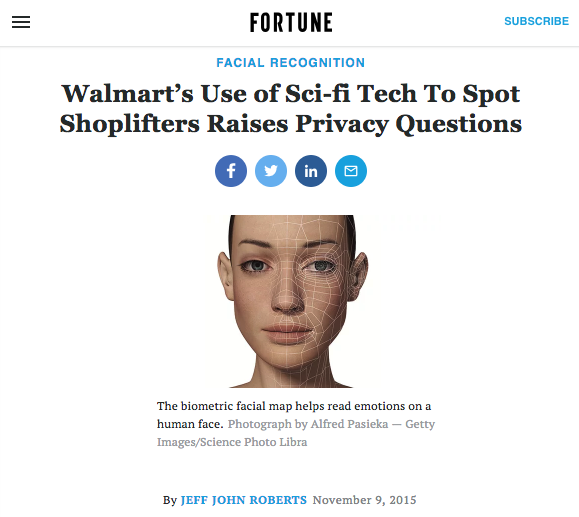
\includegraphics[width=0.8\linewidth]{Reportagem_3.png}}
\end{frame}


%FRAME%%%%%%%%%%%%%%%%%%%%%%%%%%%%%%%%%%%%%%%%%%%%%%%
\begin{frame}
    \centerline{\noindent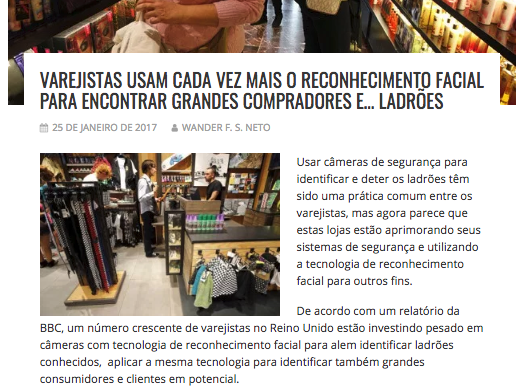
\includegraphics[width=0.8\linewidth]{Reportagem_2.png}}
\end{frame}


%FRAME%%%%%%%%%%%%%%%%%%%%%%%%%%%%%%%%%%%%%%%%%%%%%%%
\begin{frame}
    \centerline{\noindent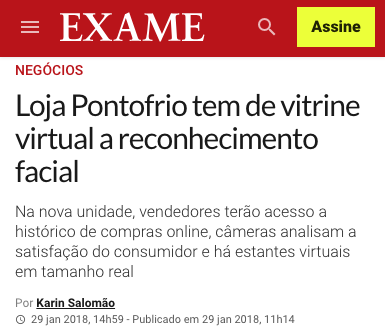
\includegraphics[width=0.8\linewidth]{Reportagem_1.png}}
\end{frame}

%FRAME%%%%%%%%%%%%%%%%%%%%%%%%%%%%%%%%%%%%%%%%%%%%%%%
\begin{frame}
    \centerline{\noindent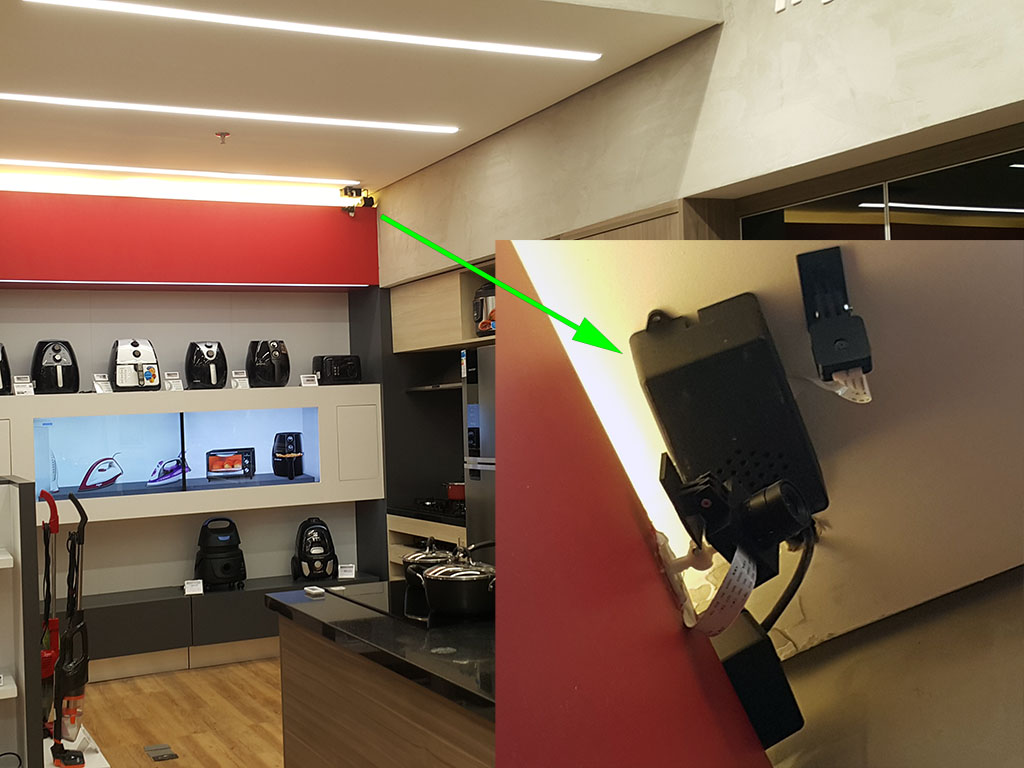
\includegraphics[width=0.8\linewidth]{imagens/ponto_frio_camera.jpg}}
\end{frame}

%SUBSEC%%%%%%%%%%%%%%%%%%%%%%%%%%%%%%%%%%%%%%%%%%%%%%%
\subsection{Objetivos}

%FRAME%%%%%%%%%%%%%%%%%%%%%%%%%%%%%%%%%%%%%%%%%%%%%%%
\begin{frame}{Objetivos}
%Os objetivos deste trabalho são:
\begin{itemize}
    \item Fornecer uma base teórica e prática para a construção de um sistema de detecção e reconhecimento facial, que será utilizado em uma loja de varejo
    \item Encontrar bibliotecas, APIs e ferramentas que auxiliem no desenvolvimento do projeto
\end{itemize}
\end{frame}


%FRAME%%%%%%%%%%%%%%%%%%%%%%%%%%%%%%%%%%%%%%%%%%%%%%%
\begin{frame}{Aplicações}
Aplicações de detecção e reconhecimento facial:
\medskip
\begin{itemize}
    \item Identificação criminal
    \item Sistemas de segurança
    \item Biometria
    \item Processamento de imagens
    \item Interação humano-computador
\end{itemize}
\end{frame}

%FRAME%%%%%%%%%%%%%%%%%%%%%%%%%%%%%%%%%%%%%%%%%%%%%%%
\begin{frame}{Exemplo}
\centerline{\noindent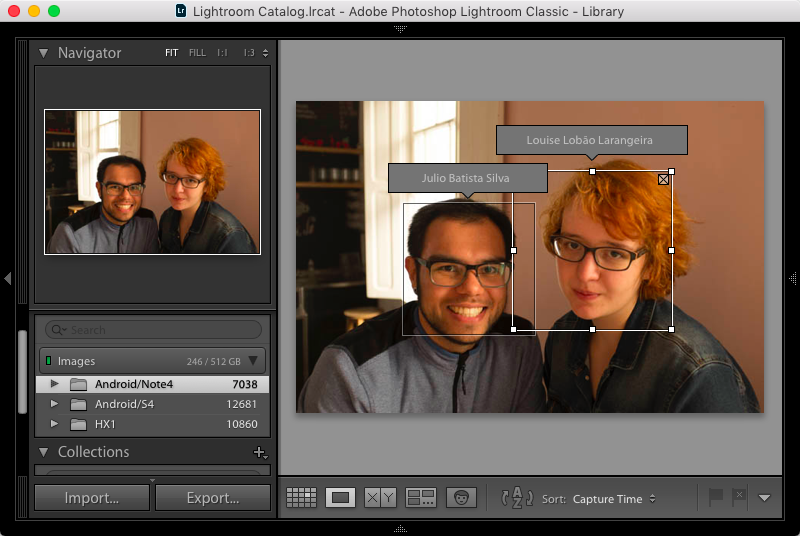
\includegraphics[width=0.9\linewidth]{lightroom_reconhecimento.png}}
\end{frame}

%FRAME%%%%%%%%%%%%%%%%%%%%%%%%%%%%%%%%%%%%%%%%%%%%%%%
\begin{frame}{Nem sempre funciona como esperado}
\centerline{\noindent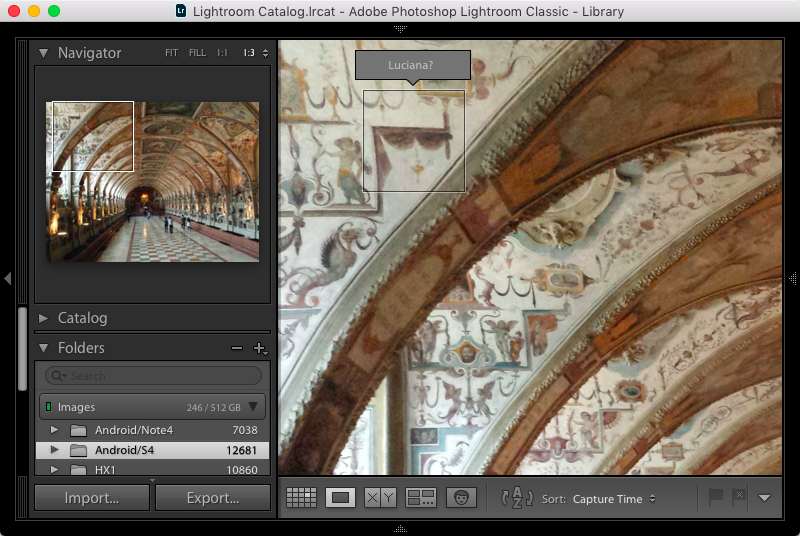
\includegraphics[width=0.9\linewidth]{lightroom_erro.png}}
\end{frame}


%FRAME%%%%%%%%%%%%%%%%%%%%%%%%%%%%%%%%%%%%%%%%%%%%%%%
\begin{frame}{Dificuldades}
\begin{overprint}
\begin{figure}
\centering

% Imagens de cima
\only<1-5>{\begin{minipage}{0.31\textwidth}
  \caption{Iluminação}
  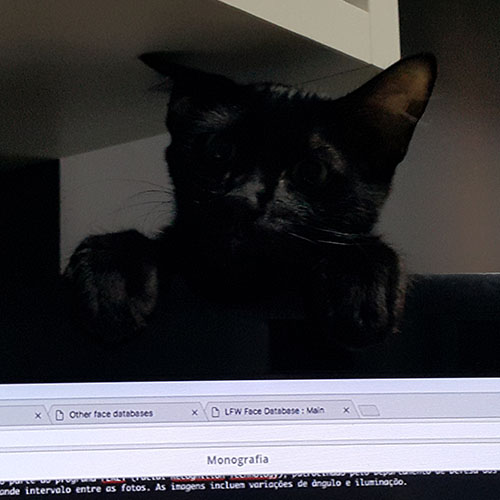
\includegraphics[width=0.8\textwidth]{imagens/iluminacao_01.jpg}
\end{minipage}}
\only<2-5>{\begin{minipage}{0.31\textwidth}
    \centering
    \caption{Pose}
    \label{fig:oclusao}
    \begin{subfigure}[t]{0.5\textwidth}
    \centering
    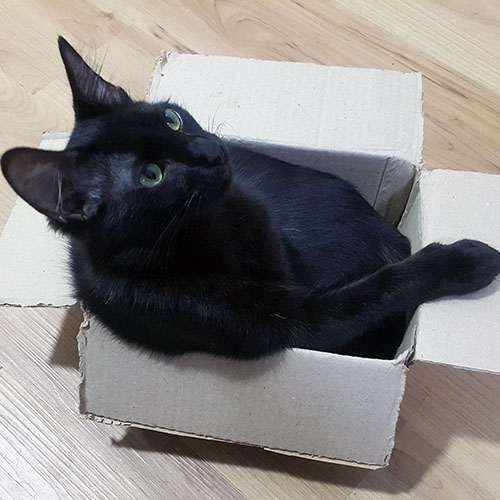
\includegraphics[width=0.8\linewidth]{imagens/pose_01.jpg}
    \end{subfigure}
    \begin{subfigure}[t]{0.5\textwidth}
    \centering
    
\includegraphics[width=0.8\linewidth]{imagens/pose_02.jpg}
    \end{subfigure}
\end{minipage}}

% Imagens de baixo
\only<3-5>{\begin{minipage}{0.31\textwidth}
    \centering
    \caption{Expressão Facial}
    \label{fig:expressao_facial}
    \begin{subfigure}[t]{0.5\textwidth}
    \centering
    
\includegraphics[width=0.85\linewidth]{imagens/expressao_01.jpg}
    \end{subfigure}
    \begin{subfigure}[t]{0.5\textwidth}
    \centering
    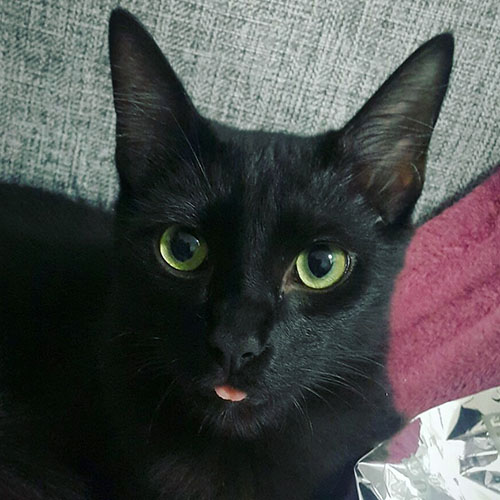
\includegraphics[width=0.85\linewidth]{imagens/expressao_02.jpg}
    \end{subfigure}
\end{minipage}}
\only<4-5>{\begin{minipage}{0.31\textwidth}
    \centering
    \caption{Oclusão}
    \label{fig:oclusao}
    \begin{subfigure}[t]{0.5\textwidth}
    \centering
    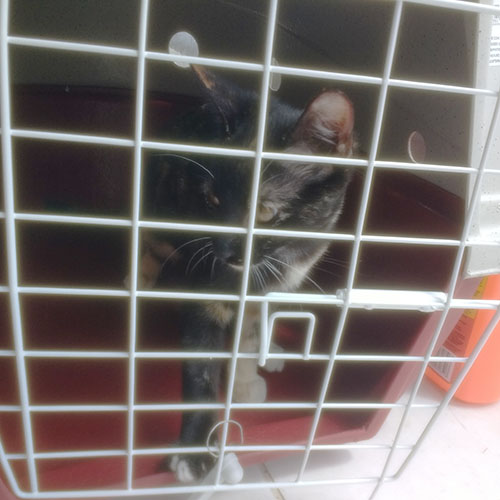
\includegraphics[width=0.85\linewidth]{imagens/oclusao_01.jpg}
    \end{subfigure}
    \begin{subfigure}[t]{0.5\textwidth}
    \centering
    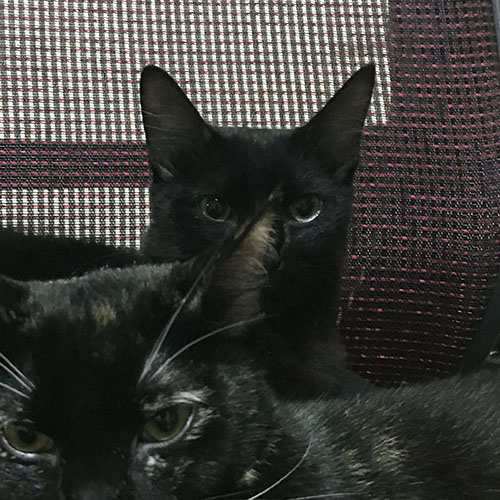
\includegraphics[width=0.85\linewidth]{imagens/oclusao_02.jpg}
    \end{subfigure}
\end{minipage}}
\only<5>{\begin{minipage}{0.31\textwidth}
    \centering
    \caption{Ponto de Vista}
    \label{fig:ponto_vista}
    \begin{subfigure}[t]{0.5\textwidth}
    \centering
    
\includegraphics[width=0.85\linewidth]{imagens/ponto_vista_01.jpg}
    \end{subfigure}
    \begin{subfigure}[t]{0.5\textwidth}
    \centering
    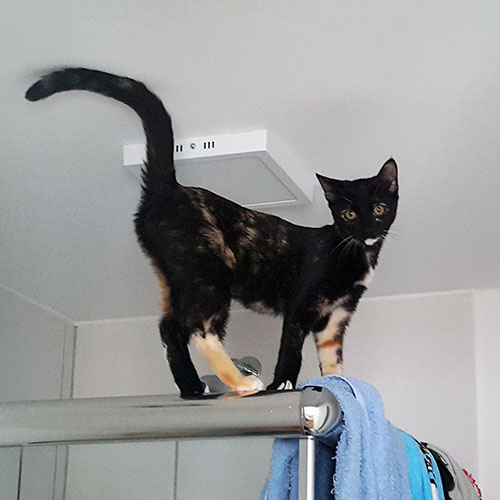
\includegraphics[width=0.85\linewidth]{imagens/ponto_vista_02.jpg}
    \end{subfigure}
\end{minipage}}
\end{figure}
\end{overprint}\end{frame}
%%%%%%%%%%%%%%%%%%%%%%%%%%%%%%%%%%%%%%%%%%%%%%%%%%%%%%
%SEC%%%%%%%%%%%%%%%%%%%%%%%%%%%%%%%%%%%%%%%%%%%%%%%%%%
\section{Detecção Facial}

%FRAME%%%%%%%%%%%%%%%%%%%%%%%%%%%%%%%%%%%%%%%%%%%%%%%
\begin{frame}{Definição}
O papel de um detector de faces é, dada uma imagem arbitrária, determinar se ela contém faces ou não e, caso positivo, retornar a localização e dimensões de cada face \cite{censtudy}
\end{frame}


%FRAME%%%%%%%%%%%%%%%%%%%%%%%%%%%%%%%%%%%%%%%%%%%%%%%
\begin{frame}{}
\begin{figure}[htbp]
    \caption{Fonte: \citeonline{nikons60ad}}
    \label{fig:nikon}
    \begin{center}
        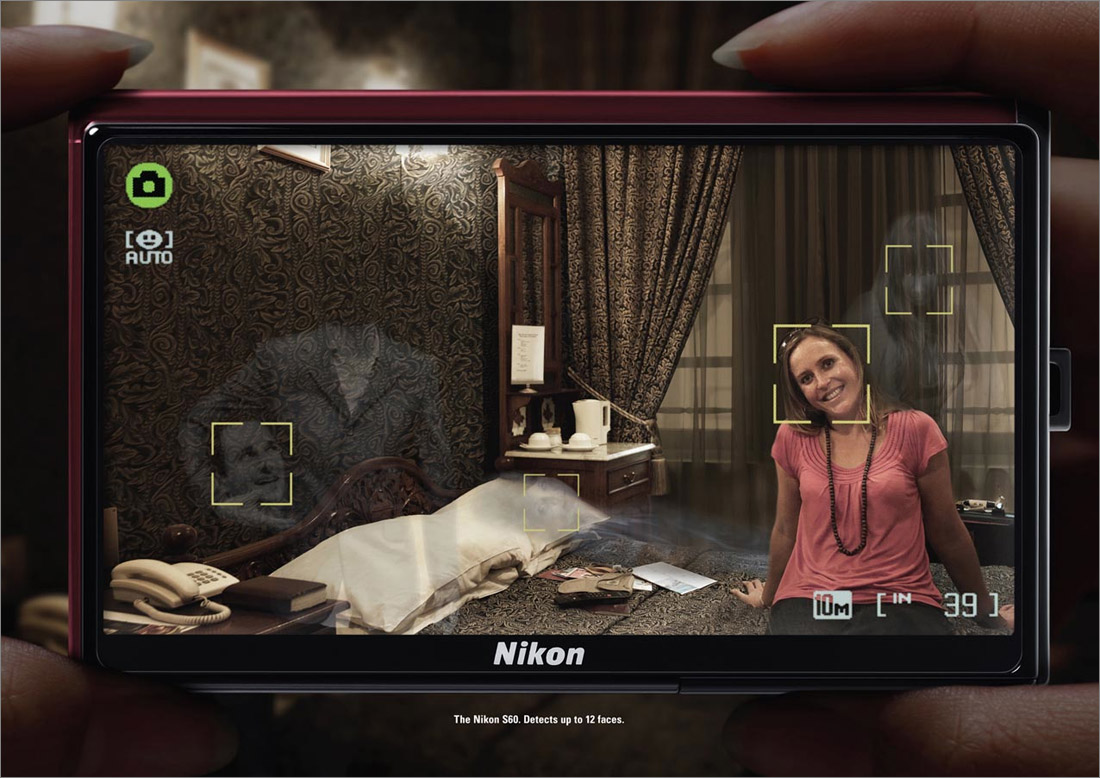
\includegraphics[width=0.9\linewidth]{imagens/nikon_s60_3.jpg}
    \end{center}
\end{figure}
\end{frame}


%FRAME%%%%%%%%%%%%%%%%%%%%%%%%%%%%%%%%%%%%%%%%%%%%%%%
%\begin{frame}{Métodos}
%\begin{figure}[htbp]
%    \label{fig:metodos_deteccao}
%    \begin{subfigure}[t]{0.45\textwidth}
%    \centering
%    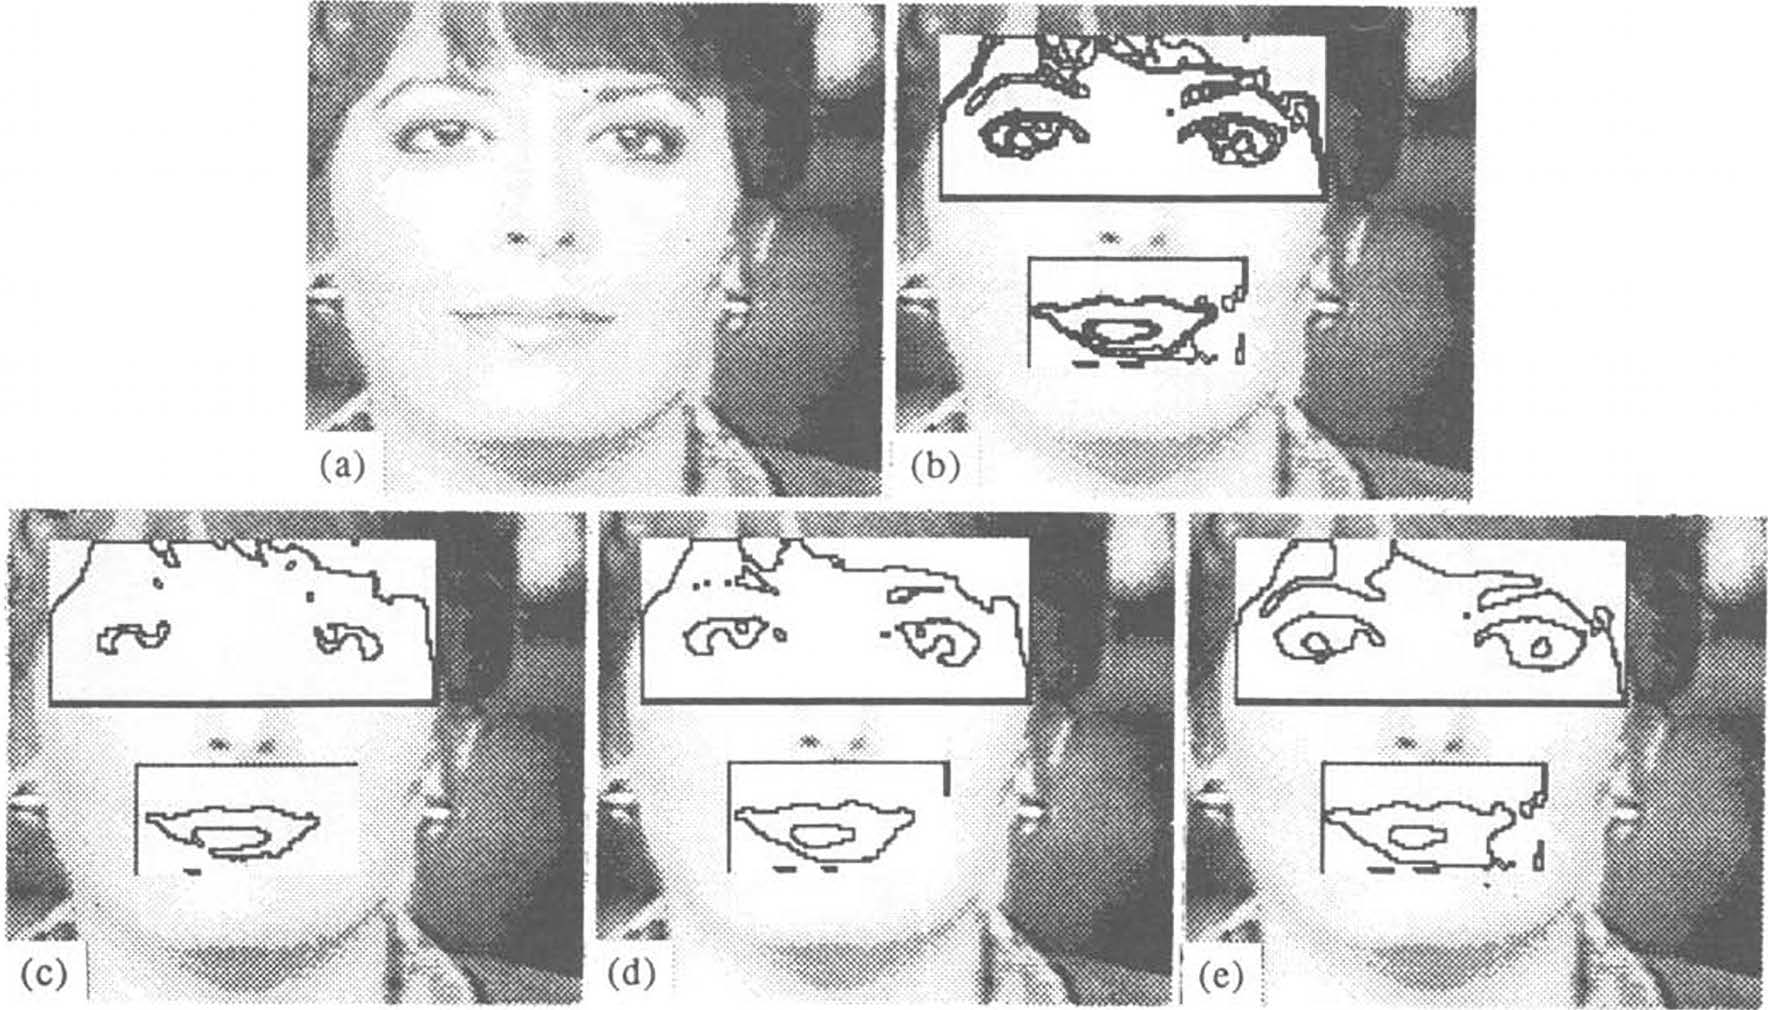
\includegraphics[width=0.7\textwidth]{imagens/yang_edge_detection.png}
%    \caption{Baseado em conhecimento. Fonte: \citeonline{yang1994human}}
%    \end{subfigure}
%    \hfill
%    \begin{subfigure}[t]{0.45\textwidth}
%    \centering
%    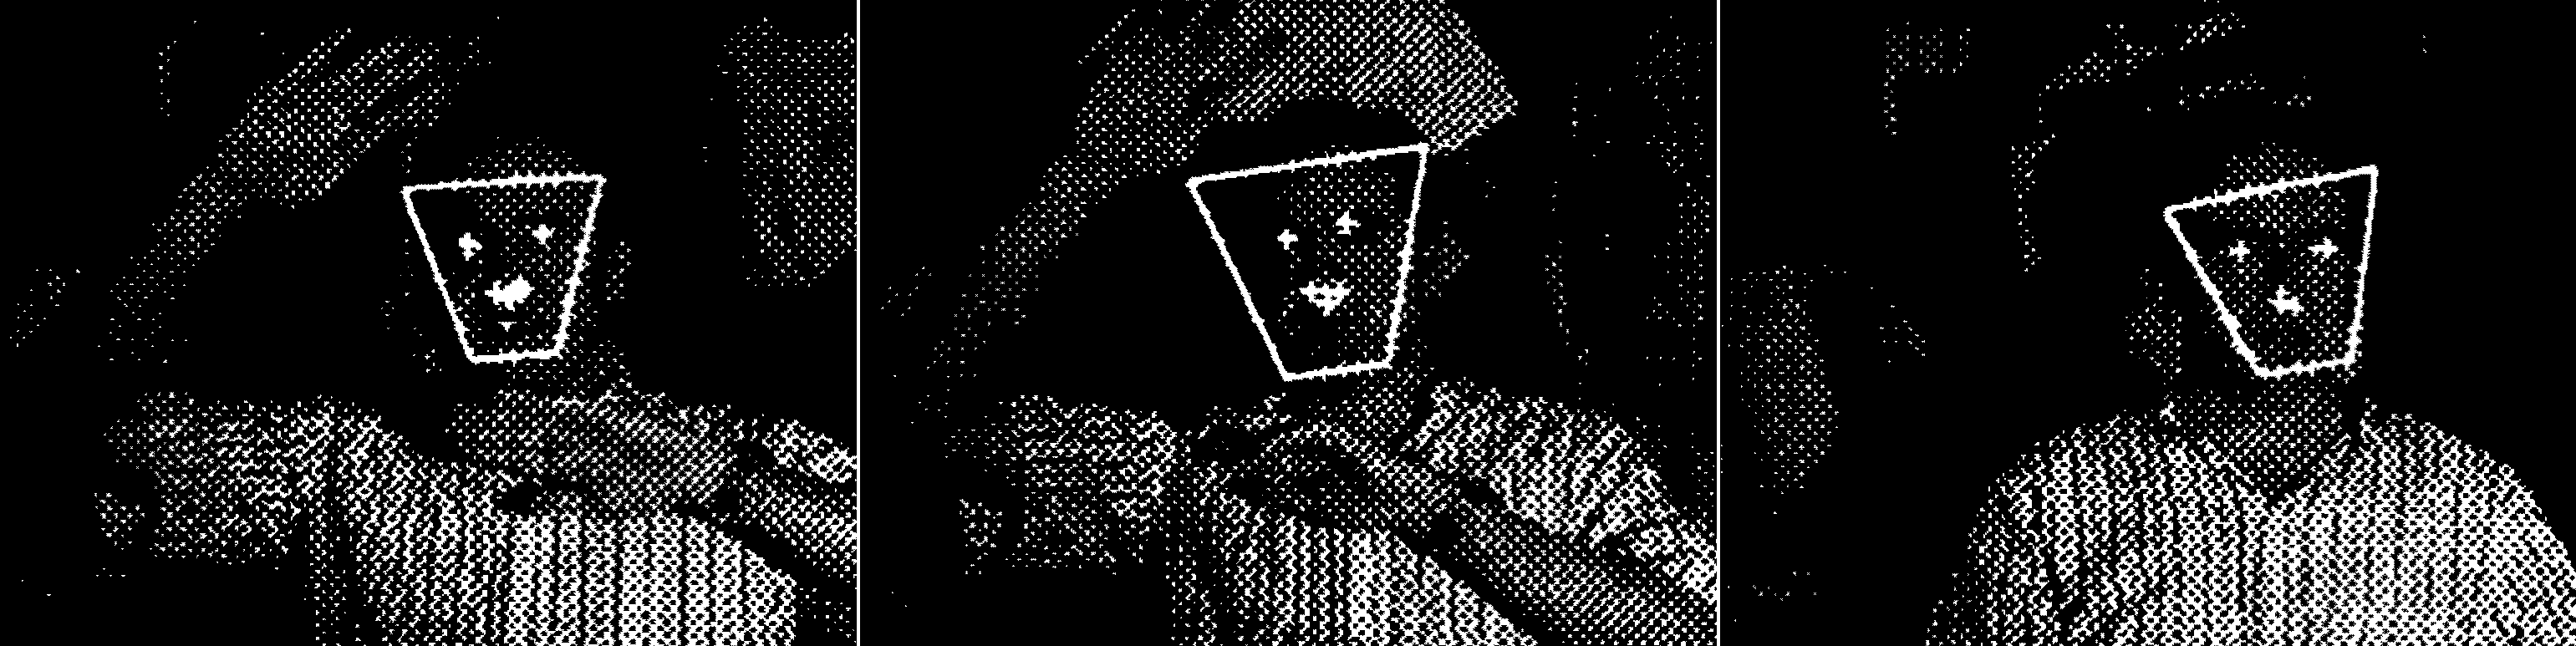
\includegraphics[width=0.7\textwidth]{imagens/leung.png}
%    \caption{Baseado em características invariantes.  Fonte: \citeonline{leung1995finding}}
%    \end{subfigure}
%    
%    \begin{subfigure}[t]{0.45\textwidth}
%    \centering
%    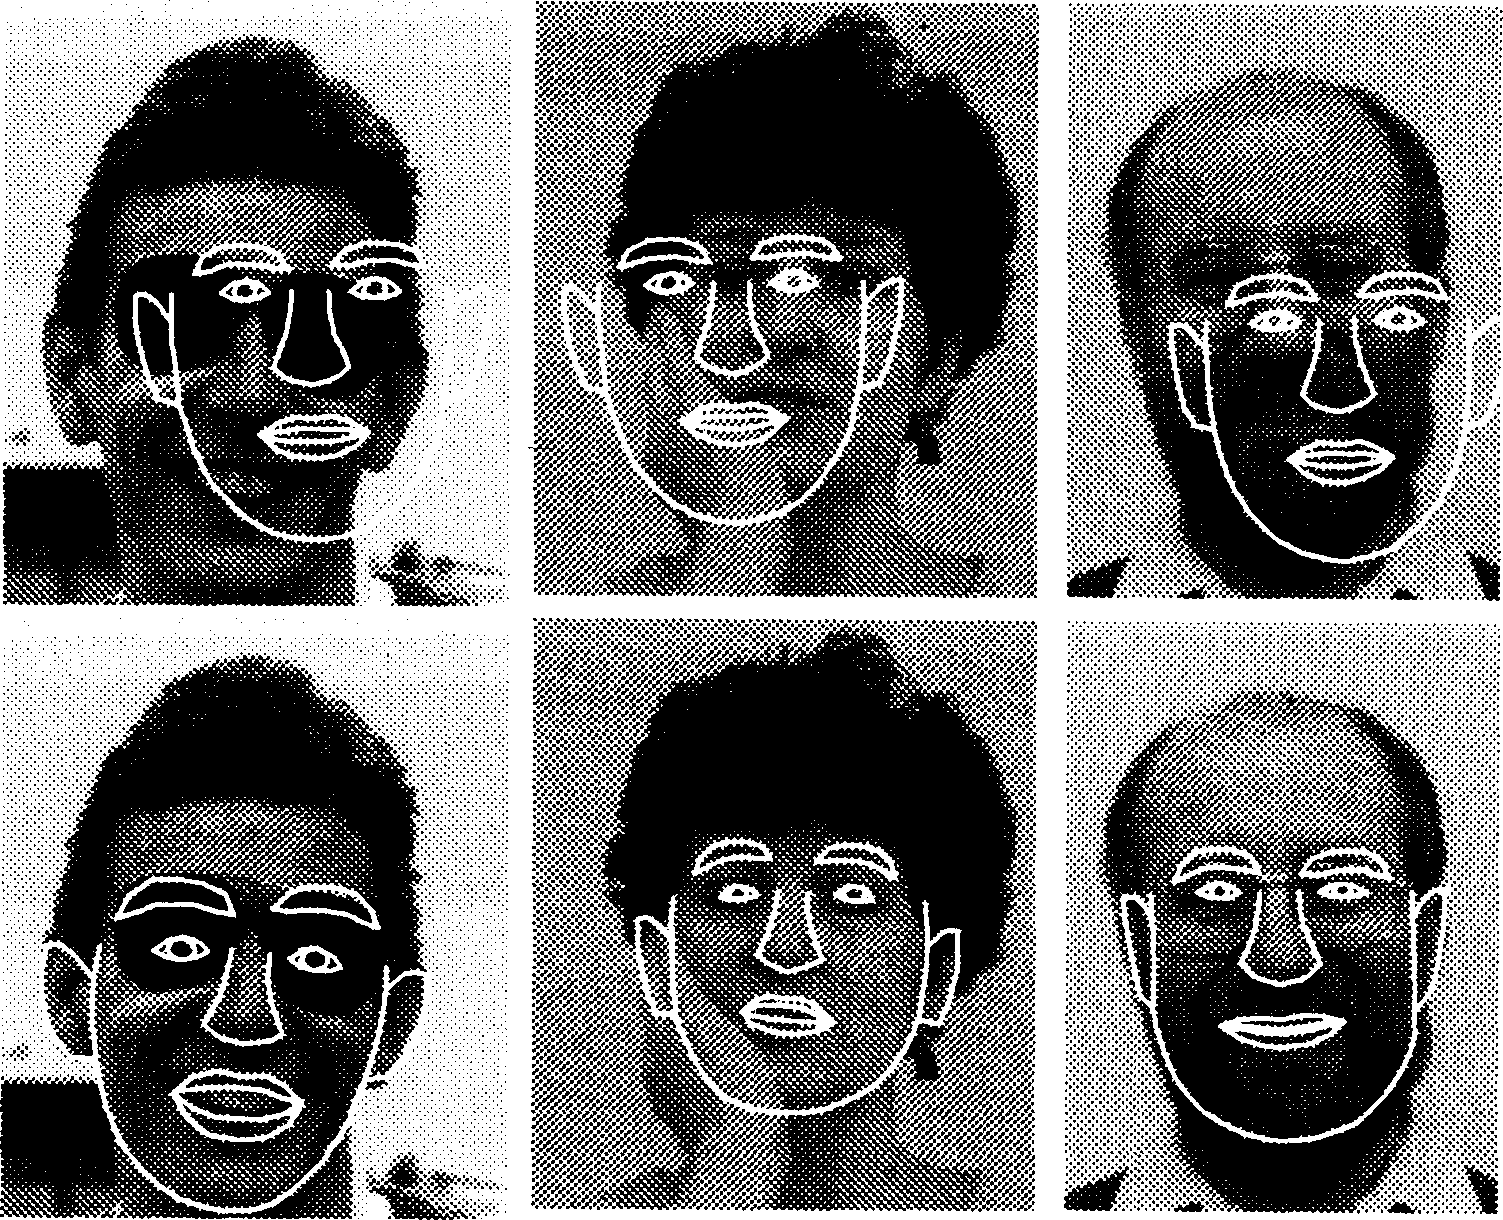
\includegraphics[width=0.6\textwidth]{imagens/lanitis_template.png}
%    \caption{Casamento de padrões. Fonte: \citeonline{lanitis1995automatic}}
%    \end{subfigure}
%    \hfill
%    \begin{subfigure}[t]{0.45\textwidth}
%    \centering
%    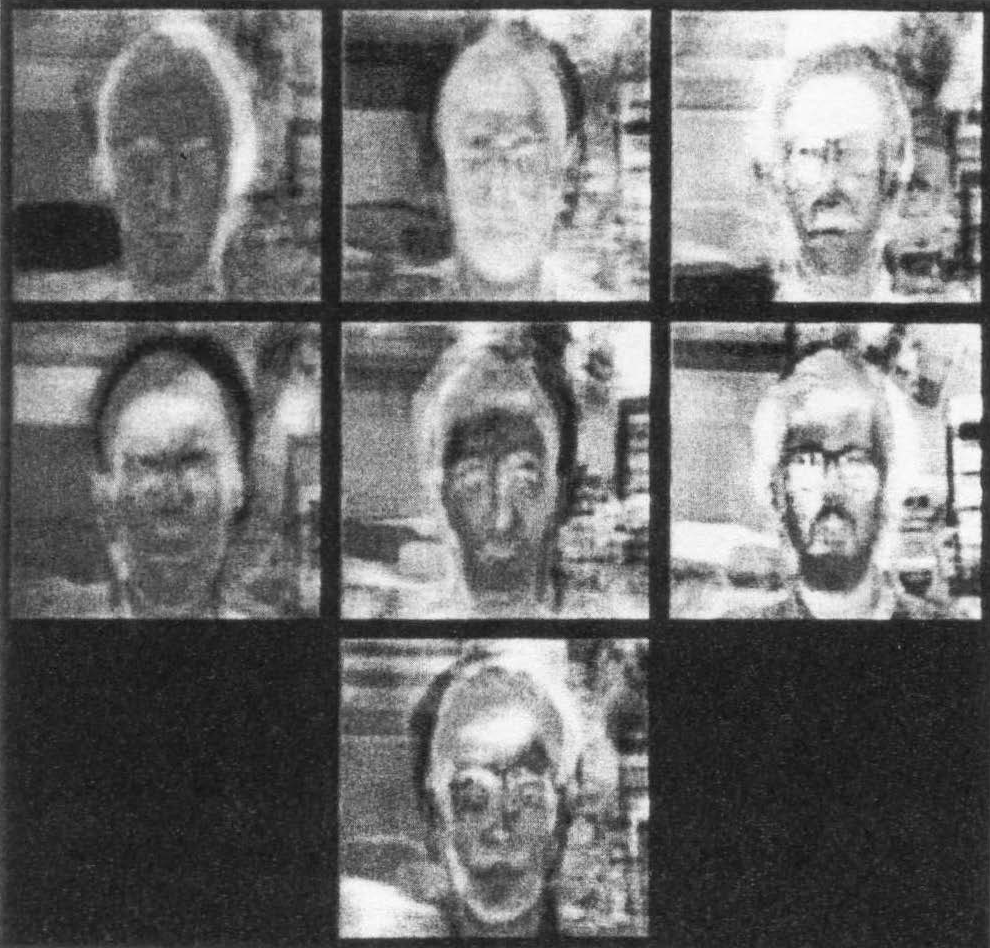
\includegraphics[width=0.6\textwidth]{imagens/turk_eigenfaces.png}
%    \caption{Baseado na aparência. Fonte: \citeonline{turk1991eigenfaces}}
%    \end{subfigure}
%\end{figure}
%\end{frame}


%FRAME%%%%%%%%%%%%%%%%%%%%%%%%%%%%%%%%%%%%%%%%%%%%%%%
\begin{frame}{Métodos}
\begin{itemize}
    \item Baseado em conhecimento
\end{itemize}

\begin{figure}[htbp]
    \centering
    \caption{Fonte: \citeonline{yang1994human}}
    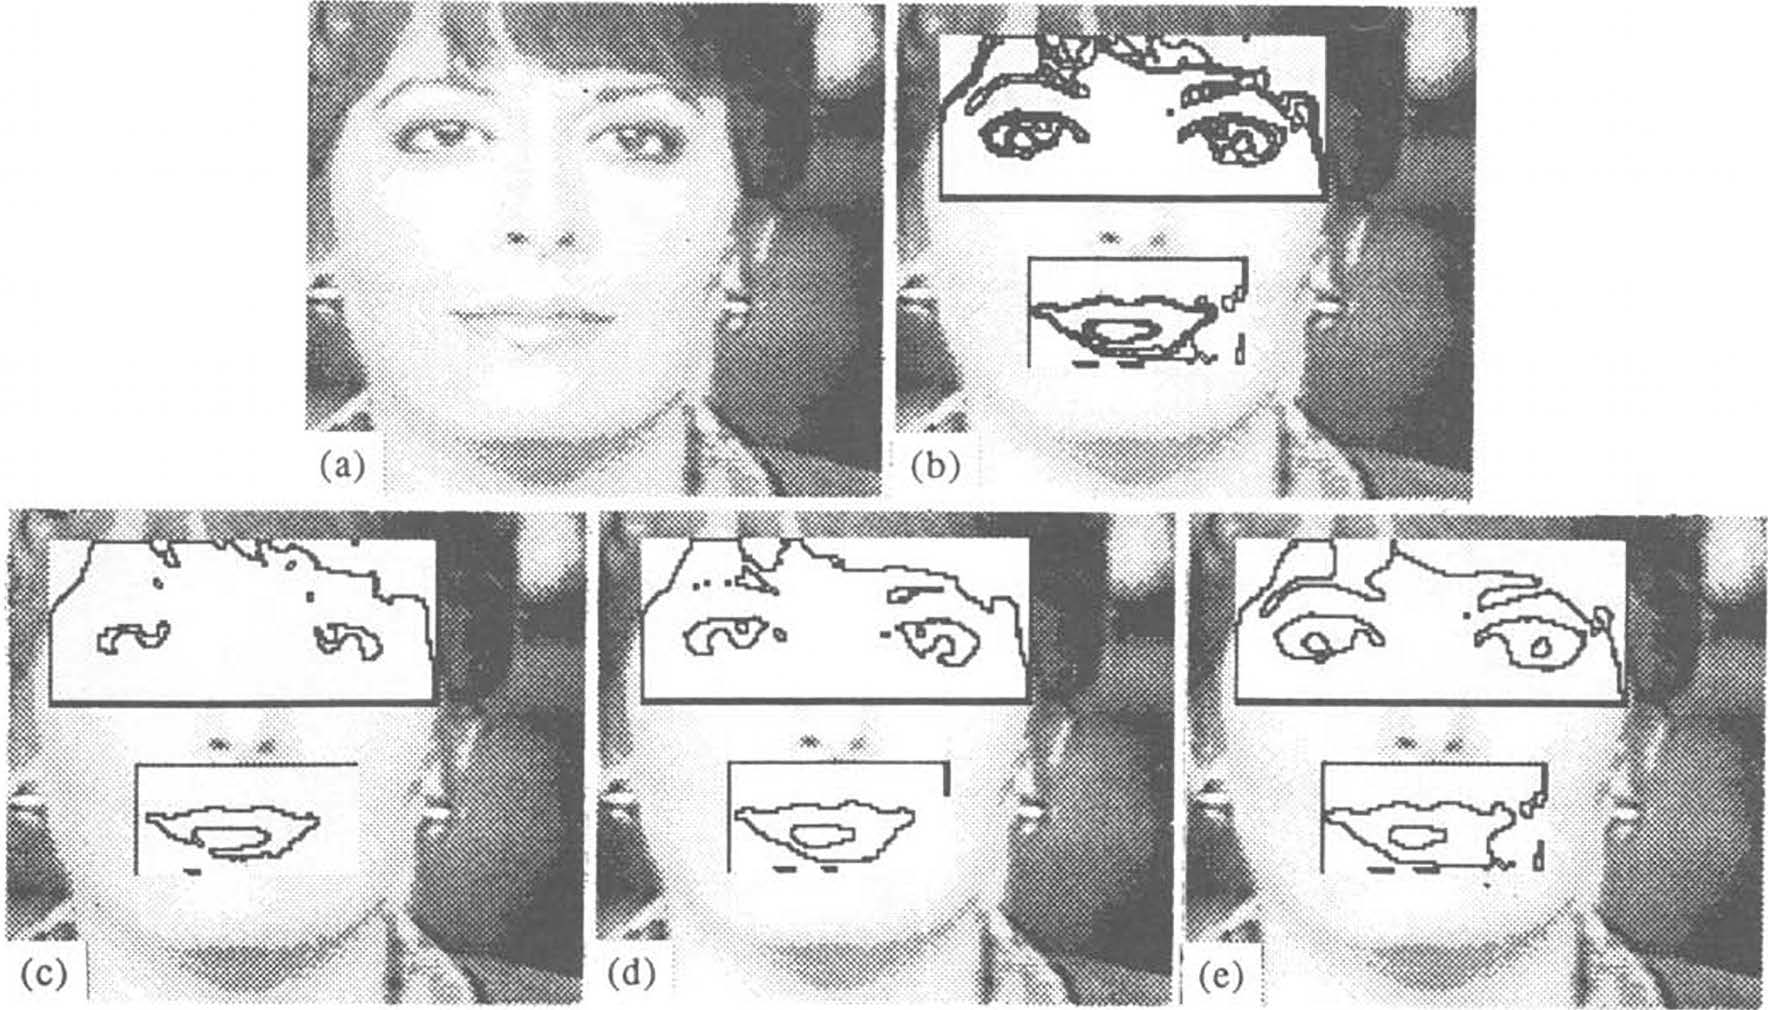
\includegraphics[height=0.6\textheight]{imagens/yang_edge_detection.png}
\end{figure}
\end{frame}


%FRAME%%%%%%%%%%%%%%%%%%%%%%%%%%%%%%%%%%%%%%%%%%%%%%%
\begin{frame}{Métodos}
\begin{itemize}
    \item Baseado em características invariantes
\end{itemize}

\begin{figure}[htbp]
    \caption{Fonte: \citeonline{leung1995finding}}
    \centering
    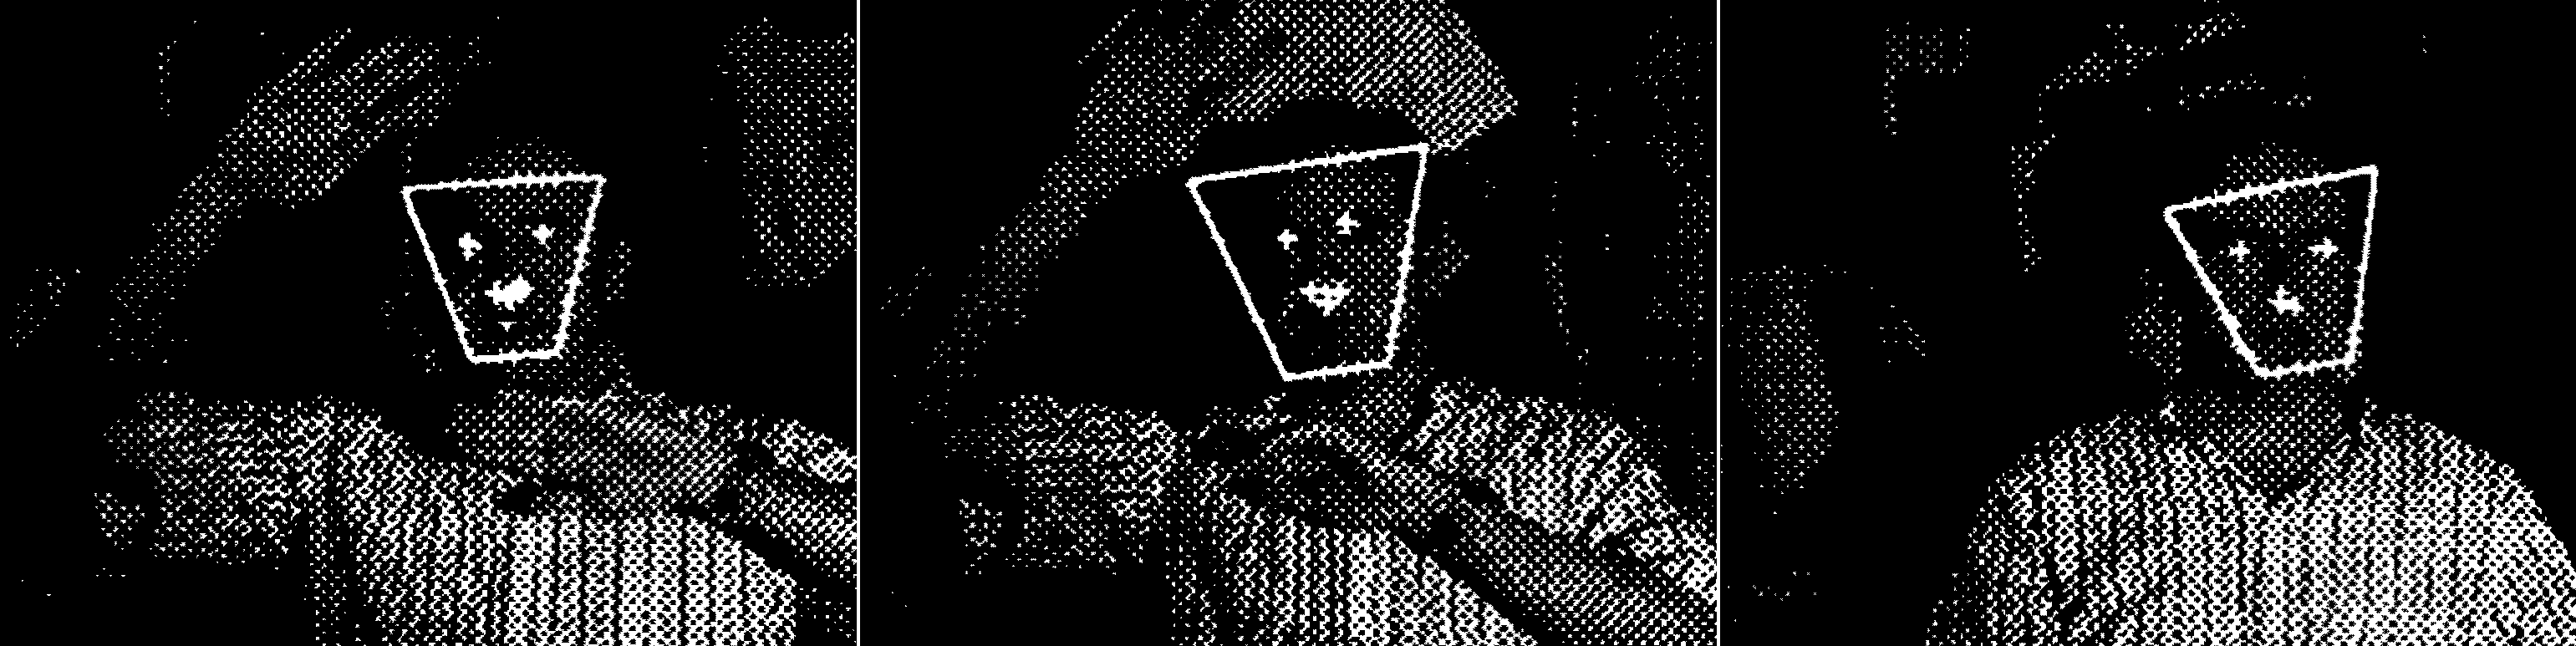
\includegraphics[height=0.6\textheight,width=\textwidth]{imagens/leung.png}
\end{figure}
\end{frame}


%FRAME%%%%%%%%%%%%%%%%%%%%%%%%%%%%%%%%%%%%%%%%%%%%%%%
\begin{frame}{Métodos}
\begin{itemize}
    \item Casamento de padrões
\end{itemize}

\begin{figure}[htbp]
    \caption{Fonte: \citeonline{lanitis1995automatic}}
    \centering
    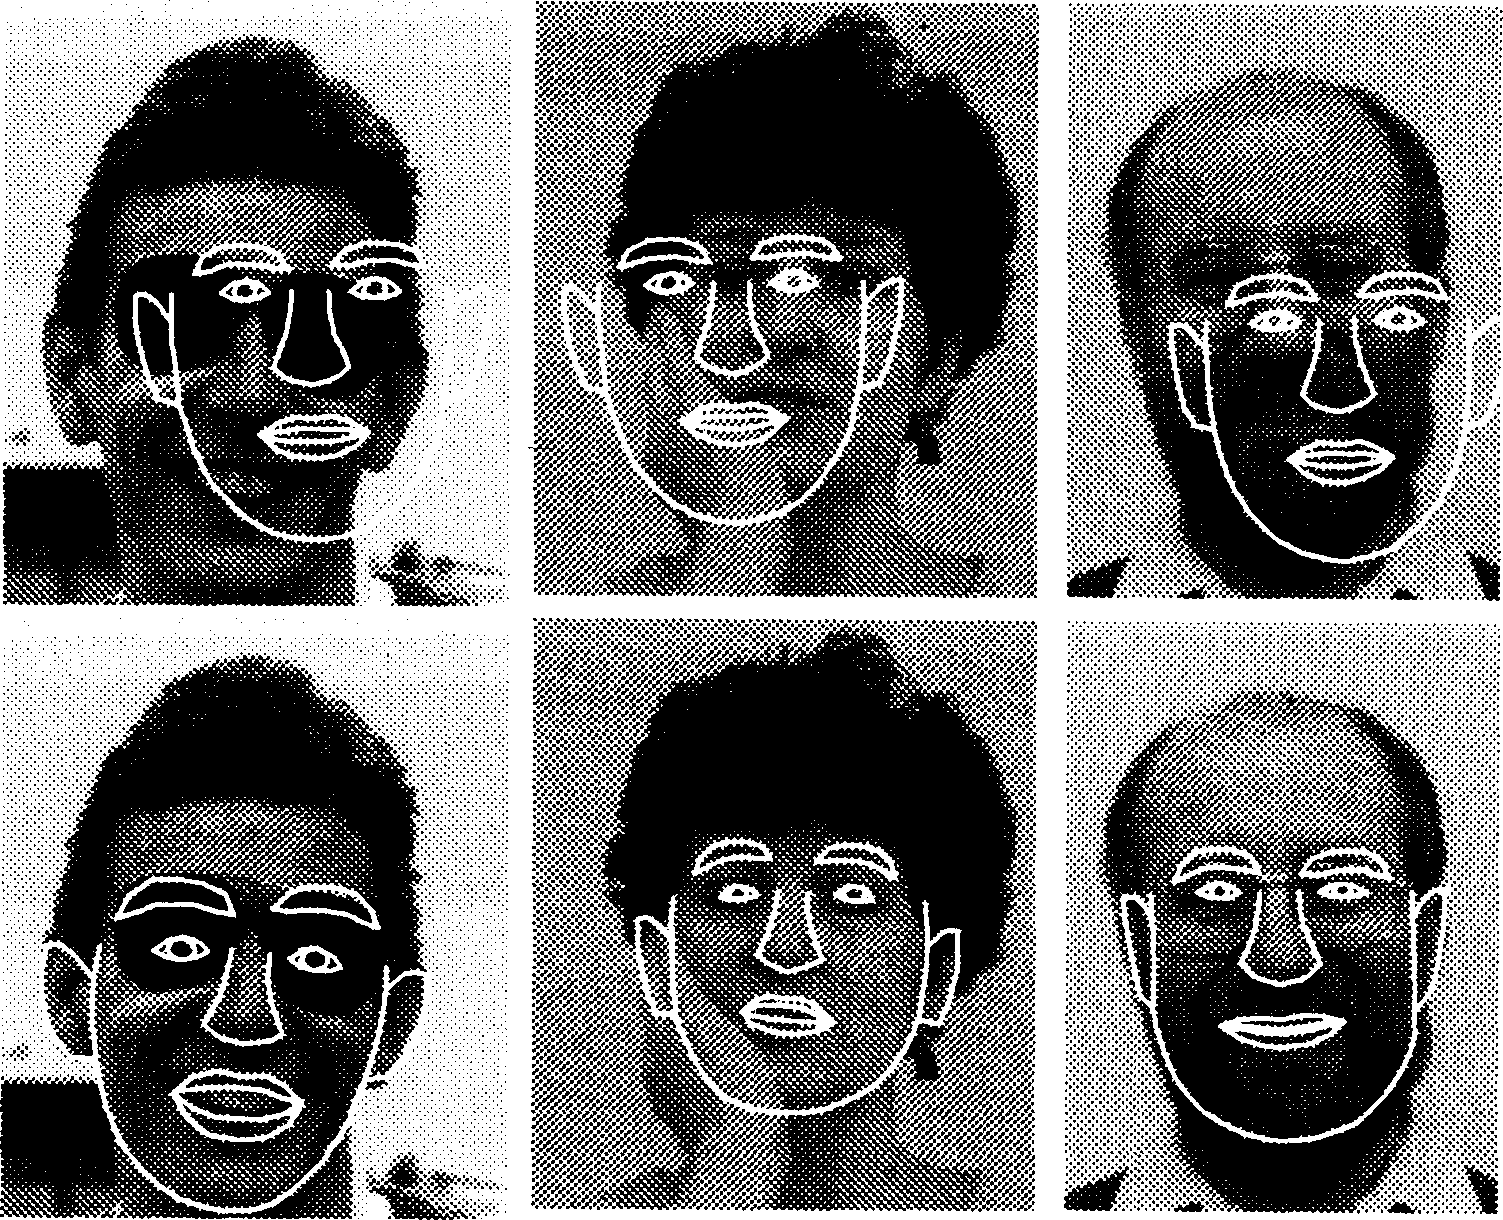
\includegraphics[height=0.6\textheight]{imagens/lanitis_template.png}
\end{figure}
\end{frame}


%FRAME%%%%%%%%%%%%%%%%%%%%%%%%%%%%%%%%%%%%%%%%%%%%%%%
\begin{frame}{Métodos}
\begin{itemize}
    \item Baseado na aparência
\end{itemize}

\begin{figure}
    \caption{Fonte: \citeonline{turk1991eigenfaces}}
    \centering
    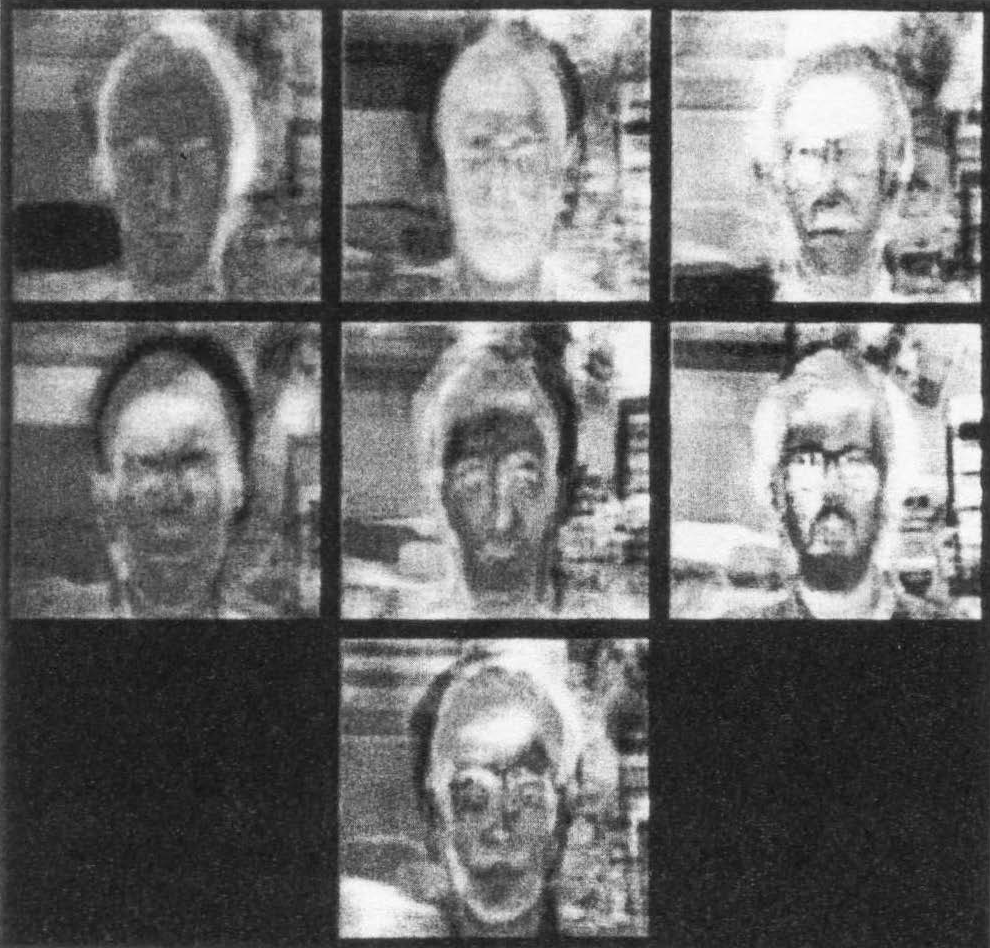
\includegraphics[height=0.6\textheight]{imagens/turk_eigenfaces.png}
\end{figure}
\end{frame}


%SUBSEC%%%%%%%%%%%%%%%%%%%%%%%%%%%%%%%%%%%%%%%%%%%%%%%
\subsection{Viola-Jones}

%FRAME%%%%%%%%%%%%%%%%%%%%%%%%%%%%%%%%%%%%%%%%%%%%%%%
\begin{frame}{Viola-Jones}
\begin{itemize}
    \item Algoritmo apresentado por Paul Viola e Michael Jones em 2001 \cite{Viola01rapidobject}
    \item Foi o primeiro método de detecção de faces em tempo real \citeonline{omaia2009sistema}
\end{itemize}
\end{frame}

%FRAME%%%%%%%%%%%%%%%%%%%%%%%%%%%%%%%%%%%%%%%%%%%%%%%
\begin{frame}{Viola-Jones}
\begin{itemize}
    \item Não é apenas para faces humanas
\end{itemize}

\begin{figure}
    \centering
    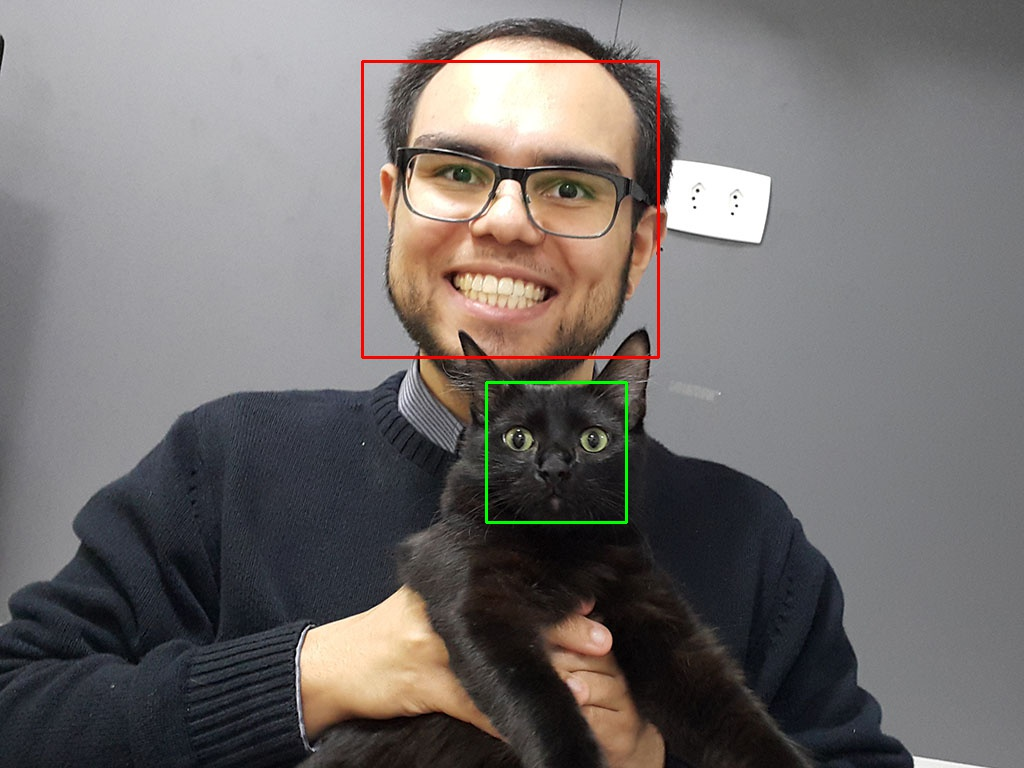
\includegraphics[width=0.8\textwidth]{imagens/detecta_joca.jpg}
\end{figure}
\end{frame}

%FRAME%%%%%%%%%%%%%%%%%%%%%%%%%%%%%%%%%%%%%%%%%%%%%%%
\begin{frame}{Viola-Jones}
Quatro estágios:
\medskip
\begin{itemize}
    \item Seleção de características Haar-like retangulares
    \item Criação da imagem integral
    \item Treino de classificadores por AdaBoost
    \item Uso de classificadores em cascata
\end{itemize}
\end{frame}


%SUBSEC%%%%%%%%%%%%%%%%%%%%%%%%%%%%%%%%%%%%%%%%%%%%%%%
\subsubsection{Características Haar}

%FRAME%%%%%%%%%%%%%%%%%%%%%%%%%%%%%%%%%%%%%%%%%%%%%%%
\begin{frame}{Características Haar}
\begin{itemize}
    \item Formadas por dois, três ou quatro retângulos
    \item O cálculo de uma única característica é bem simples: soma das intensidades dos pixels sob os retângulos pretos menos a soma dos valores sob os retângulos brancos
\end{itemize}

\begin{figure}
    \centering
    
\includegraphics[width=0.8\textwidth]{imagens/haar_like_features.png}
\end{figure}
\end{frame}

%FRAME%%%%%%%%%%%%%%%%%%%%%%%%%%%%%%%%%%%%%%%%%%%%%%%
\begin{frame}[fragile]{Características Haar}
\begin{itemize}
    \item Compara quão próximo o caso real está do caso ideal
\end{itemize}

\begin{figure}[h]
    \begin{adjustbox}{max width=\textwidth, max height=0.25\textheight}
    \begin{minipage}{0.45\textwidth}
    \centering
    \begin{tikzpicture}
    \matrix[square matrix, text=cyan] {
        0 & 0 &|[fill=black]| 1 &|[fill=black]| 1 \\
        0 & 0 &|[fill=black]| 1 &|[fill=black]| 1 \\
        0 & 0 &|[fill=black]| 1 &|[fill=black]| 1 \\
        0 & 0 &|[fill=black]| 1 &|[fill=black]| 1 \\
    };
    \end{tikzpicture}
    \caption{Intensidades ideais}
    \end{minipage}
    \begin{minipage}{0.1\textwidth}
    \centering
    $\vpointer$
    \end{minipage}
    \begin{minipage}{0.45\textwidth}
    \centering
    \begin{tikzpicture}
    \matrix[square matrix, text=cyan] {
        |[fill=black!20]|0.2 &|[fill=black!20]| 0.2 &|[fill=black!80]| 0.8 &|[fill=black!60]| 0.6 \\
        |[fill=black!10]|0.1 &|[fill=black!30]| 0.3 &|[fill=black!60]| 0.6 &|[fill=black!80]| 0.8 \\
        |[fill=black!20]|0.2 &|[fill=black!10]| 0.1 &|[fill=black!80]| 0.8 &|[fill=black!80]| 0.8 \\
        |[fill=black!20]|0.2 &|[fill=black!10]| 0.1 &|[fill=black!60]| 0.6 &|[fill=black!90]| 0.9 \\
    };
    \end{tikzpicture}
    \caption{Valores reais}
    \end{minipage}
    \end{adjustbox}
\end{figure}

\begin{align*}
\Delta  &= \frac{1}{n}  \sum_{preto}^{n} I(x) - \frac{1}{n}  \sum_{branco}^{n} I(x)\\
        &= 0,74 - 0,18 = 0,56 \nonumber
\end{align*}

\end{frame}


%FRAME%%%%%%%%%%%%%%%%%%%%%%%%%%%%%%%%%%%%%%%%%%%%%%%
\begin{frame}{Características Haar}
\begin{itemize}
    \item Características usadas para detectar olhos e nariz
\end{itemize}

\begin{figure}[htbp]
    \begin{subfigure}[c]{0.4\textwidth}
    \centering
    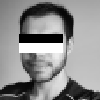
\includegraphics{imagens/julio_haar2.png}
    \end{subfigure}
    \begin{subfigure}[c]{0.4\textwidth}
    \centering
    
\includegraphics{imagens/julio_haar3.png}
    \end{subfigure}
\end{figure}
\end{frame}


%FRAME%%%%%%%%%%%%%%%%%%%%%%%%%%%%%%%%%%%%%%%%%%%%%%%
\begin{frame}{Características Haar}
Para cada subjanela de $24\times24$ pixels, seria necessário calcular 45396 características

\begin{center}{\huge Inviável!}\end{center}

\end{frame}


%SUBSUBSEC%%%%%%%%%%%%%%%%%%%%%%%%%%%%%%%%%%%%%%%%%%%%
\subsubsection{Imagem Integral}


%FRAME%%%%%%%%%%%%%%%%%%%%%%%%%%%%%%%%%%%%%%%%%%%%%%%
\begin{frame}{Imagem Integral}
\begin{itemize}
    \item Permite calcular as características em tempo constante
    \item É uma tabela onde cada elemento equivale à soma de todos os pixels à esquerda e acima do pixel atual
\end{itemize}

\begin{equation*} \label{eq:imagemintegral}
    ii(x,y) = \sum_{{x}'\leq x, {y}'\leq y} i({x}', {y}')
\end{equation*}

\end{frame}

%FRAME%%%%%%%%%%%%%%%%%%%%%%%%%%%%%%%%%%%%%%%%%%%%%%%
\begin{frame}[fragile]{Imagem Integral}

\begin{figure}[h]
    \begin{minipage}{0.44\textwidth}
    \caption{Imagem original}
    \centering
    \begin{adjustbox}{max width=\textwidth}
    \begin{tikzpicture}
    \matrix[square matrix] {
        0.1 & 0.1 & 0.2 & 0.1 & 0.7 & 0.1 \\
        0.2 & 0.3 & 0.2 & 0.7 & 0.8 & 0.2 \\
        0.1 & 0.4 & 0.3 & 0.3 & 0.1 & 0.3 \\
        0.1 & 0.5 & 0.1 & 0.1 & 0.2 & 0.8 \\
        0.1 & 0.4 & 0.8 & 0.5 & 0.6 & 0.5\\
    };
    \end{tikzpicture}
    \end{adjustbox}
    \end{minipage}
    \begin{minipage}{0.1\textwidth}
    \caption{ }
    \centering
    $\vpointer$
    \end{minipage}
    \begin{minipage}{0.44\textwidth}
    \caption{Imagem integral}
    \centering
    \begin{adjustbox}{max width=\textwidth}
    \begin{tikzpicture}
    \matrix[square matrix] {
        0.1 & 0.2 & 0.4 & 0.5 & 1.2 & 1.3 \\
        0.3 & 0.7 & 1.1 & 1.9 & 3.4 & 3.7 \\
        0.4 & 1.2 & 1.9 & 3.0 & 4.6 & 5.2 \\
        0.5 & 1.7 & 2.5 & 3.7 & 5.3 & 6.7 \\
        0.6 & 2.3 & 3.9 & 5.6 & 8.0 & 9.9 \\
    };
    \end{tikzpicture}
    \end{adjustbox}
    \end{minipage}
\end{figure}

\end{frame}


%FRAME%%%%%%%%%%%%%%%%%%%%%%%%%%%%%%%%%%%%%%%%%%%%%%%
\begin{frame}[fragile]{Imagem Integral}

\begin{figure}[h]
    \begin{minipage}{0.44\textwidth}
    \caption{Imagem original}
    \centering
    \begin{adjustbox}{max width=\textwidth}
    \begin{tikzpicture}
    \matrix[square matrix, opacity=0.2] (m){
        0.1 & 0.1 & 0.2 & 0.1 & 0.7 & 0.1 \\
        0.2 & 0.3 & 0.2 & 0.7 & 0.8 & 0.2 \\
        0.1 & 0.4 & 0.3 & 0.3 & 0.1 & 0.3 \\
        0.1 & 0.5 & 0.1 & 0.1 & 0.2 & 0.8 \\
        0.1 & 0.4 & 0.8 & 0.5 & 0.6 & 0.5 \\
    };
    \filldraw[fill=black!50, fill opacity=0.2, text opacity=1] (m-1-1.north west) rectangle (m-1-2.south east) node[pos=.5] {A};
    \filldraw[fill=black!70, fill opacity=0.2, text opacity=1] (m-1-3.north west) rectangle (m-1-4.south east) node[pos=.5] {B};
    \filldraw[fill=black!90, fill opacity=0.2, text opacity=1] (m-2-1.north west) rectangle (m-4-2.south east) node[pos=.5] {C};
    \filldraw[fill=yellow, fill opacity=0.2, text opacity=1] (m-2-3.north west) rectangle (m-4-4.south east) node[pos=.5] {D};
    
    \fill[blue] (m-1-2.south east) circle(2pt) node[above right] {P1};
    \fill[blue] (m-1-4.south east) circle(2pt) node[above right] {P2};
    \fill[blue] (m-4-2.south east) circle(2pt) node[above right] {P3};
    \fill[blue] (m-4-4.south east) circle(2pt) node[above right] {P4};
    \end{tikzpicture}
    \end{adjustbox}
    \end{minipage}
    \begin{minipage}{0.1\textwidth}
    \caption{ }
    \centering
    $\vpointer$
    \end{minipage}
    \begin{minipage}{0.44\textwidth}
    \caption{Imagem integral}
    \centering
    \begin{adjustbox}{max width=\textwidth}
    \begin{tikzpicture}
    \matrix[square matrix] (m){
        0.1 & 0.2 & 0.4 & 0.5 & 1.2 & 1.3 \\
        0.3 & 0.7 & 1.1 & 1.9 & 3.4 & 3.7 \\
        0.4 & 1.2 & 1.9 & 3.0 & 4.6 & 5.2 \\
        0.5 & 1.7 & 2.5 & 3.7 & 5.3 & 6.7 \\
        0.6 & 2.3 & 3.9 & 5.6 & 8.0 & 9.9 \\
    };
    \filldraw[fill=yellow, fill opacity=0.2] (m-1-2.north west) rectangle (m-1-2.south east);
    \filldraw[fill=yellow, fill opacity=0.2] (m-1-4.north west) rectangle (m-1-4.south east);
    \filldraw[fill=yellow, fill opacity=0.2] (m-4-2.north west) rectangle (m-4-2.south east);
    \filldraw[fill=yellow, fill opacity=0.2] (m-4-4.north west) rectangle (m-4-4.south east);
    \draw[blue,<-,shorten <=1pt] (m-1-2)
    |- +(0.2,0.8)
    node[right] {$ii(P1)$};
     \draw[blue,<-,shorten <=1pt] (m-1-4)
    |- +(0.2,0.8)
    node[right] {$ii(P2)$};
    \draw[blue,<-,shorten <=1pt] (m-4-2)
    |- +(0.2,-1.4)
    node[right] {$ii(P3)$};
    \draw[blue,<-,shorten <=1pt] (m-4-4)
    |- +(0.2,-1.4)
    node[right] {$ii(P4)$};
    \end{tikzpicture}%
    \end{adjustbox}
    \end{minipage}
\end{figure}

\begin{align*}
D &= (ii(P4) + ii(P1)) - (ii(P2) + ii(P3)) \\
  &= (3,7 + 02) - (0,5 + 1,7) = 1,7 \nonumber
\end{align*}

\end{frame}



%FRAME%%%%%%%%%%%%%%%%%%%%%%%%%%%%%%%%%%%%%%%%%%%%%%%
%\begin{frame}[fragile]{Imagem Integral}
%
%Cálculo da área em amarelo
%
%\begin{figure}[h]
%    \begin{minipage}{0.44\textwidth}
%    \caption{Imagem original}
%    \centering
%    \begin{adjustbox}{max width=\textwidth}
%    \begin{tikzpicture}
%    \matrix[square matrix] {
%        |[fill=yellow!25]|0.1 & |[fill=yellow!25]|0.1 & 0.2 & 0.1 & 0.7 & 0.1 \\
%        |[fill=yellow!25]|0.2 & |[fill=yellow!25]|0.3 & 0.2 & 0.7 & 0.8 & 0.2 \\
%        |[fill=yellow!25]|0.1 & |[fill=yellow!25]|0.4 & 0.3 & 0.3 & 0.1 & 0.3 \\
%        0.1 & 0.5 & 0.1 & 0.1 & 0.2 & 0.8 \\
%        0.1 & 0.4 & 0.8 & 0.5 & 0.6 & 0.5\\
%    };
%    \end{tikzpicture}
%    \end{adjustbox}
%    \end{minipage}
%    \begin{minipage}{0.1\textwidth}
%    \caption{ }
%    \centering
%    $\vpointer$
%    \end{minipage}
%    \begin{minipage}{0.44\textwidth}
%    \caption{Imagem integral}
%    \centering
%    \begin{adjustbox}{max width=\textwidth}
%    \begin{tikzpicture}
%    \matrix[square matrix] {
%        0.1 & 0.2 & 0.4 & 0.5 & 1.2 & 1.3 \\
%        0.3 & 0.7 & 1.1 & 1.9 & 3.4 & 3.7 \\
%        0.4 &|[fill=yellow!25]| 1.2 & 1.9 & 3.0 & 4.6 & 5.2 \\
%        0.5 & 1.7 & 2.5 & 3.7 & 5.3 & 6.7 \\
%        0.6 & 2.3 & 3.9 & 5.6 & 8.0 & 9.9 \\
%    };
%    \end{tikzpicture}
%    \end{adjustbox}
%    \end{minipage}
%\end{figure}
%
%\end{frame}


%FRAME%%%%%%%%%%%%%%%%%%%%%%%%%%%%%%%%%%%%%%%%%%%%%%%
\begin{frame}[fragile]{Imagem Integral}

\begin{figure}[h]
    \begin{minipage}{0.44\textwidth}
    \caption{Imagem original}
    \centering
    \begin{adjustbox}{max width=\textwidth}
    \begin{tikzpicture}
    \matrix[square matrix] {
        |[fill=yellow!25]|0.1 & |[fill=yellow!25]|0.1 & |[fill=yellow!25]|0.2 &|[fill=yellow!25]| 0.1 & 0.7 & 0.1 \\
        |[fill=yellow!25]|0.2 & |[fill=yellow!25]|0.3 & |[fill=yellow!25]|0.2 & |[fill=yellow!25]|0.7 & 0.8 & 0.2 \\
        |[fill=yellow!25]|0.1 & |[fill=yellow!25]|0.4 & |[fill=yellow!25]|0.3 & |[fill=yellow!25]|0.3 & 0.1 & 0.3 \\
        |[fill=yellow!25]|0.1 & |[fill=yellow!25]|0.5 & |[fill=yellow!25]|0.1 & |[fill=yellow!25]|0.1 & 0.2 & 0.8 \\
        0.1 & 0.4 & 0.8 & 0.5 & 0.6 & 0.5\\
    };
    \end{tikzpicture}
    \end{adjustbox}
    \end{minipage}
    \begin{minipage}{0.1\textwidth}
    \caption{ }
    \centering
    $\vpointer$
    \end{minipage}
    \begin{minipage}{0.44\textwidth}
    \caption{Imagem integral}
    \centering
    \begin{adjustbox}{max width=\textwidth}
    \begin{tikzpicture}
    \matrix[square matrix] {
        0.1 & 0.2 & 0.4 & 0.5 & 1.2 & 1.3 \\
        0.3 & 0.7 & 1.1 & 1.9 & 3.4 & 3.7 \\
        0.4 & 1.2 & 1.9 & 3.0 & 4.6 & 5.2 \\
        0.5 & 1.7 & 2.5 &|[fill=yellow!25]|3.7 & 5.3 & 6.7 \\
        0.6 & 2.3 & 3.9 & 5.6 & 8.0 & 9.9 \\
    };
    \end{tikzpicture}
    \end{adjustbox}
    \end{minipage}
\end{figure}

\end{frame}


%FRAME%%%%%%%%%%%%%%%%%%%%%%%%%%%%%%%%%%%%%%%%%%%%%%%
\begin{frame}[fragile]{Imagem Integral}

\begin{figure}[h]
    \begin{minipage}{0.44\textwidth}
    \caption{Imagem original}
    \centering
    \begin{adjustbox}{max width=\textwidth}
    \begin{tikzpicture}
    \matrix[square matrix] {
        |[fill=red!25]|0.1 & |[fill=red!25]|0.1 & |[fill=red!25]|0.2 &|[fill=red!25]| 0.1 & 0.7 & 0.1 \\
        |[fill=yellow!25]|0.2 & |[fill=yellow!25]|0.3 & |[fill=yellow!25]|0.2 & |[fill=yellow!25]|0.7 & 0.8 & 0.2 \\
        |[fill=yellow!25]|0.1 & |[fill=yellow!25]|0.4 & |[fill=yellow!25]|0.3 & |[fill=yellow!25]|0.3 & 0.1 & 0.3 \\
        |[fill=yellow!25]|0.1 & |[fill=yellow!25]|0.5 & |[fill=yellow!25]|0.1 & |[fill=yellow!25]|0.1 & 0.2 & 0.8 \\
        0.1 & 0.4 & 0.8 & 0.5 & 0.6 & 0.5\\
    };
    \end{tikzpicture}
    \end{adjustbox}
    \end{minipage}
    \begin{minipage}{0.1\textwidth}
    \caption{ }
    \centering
    $\vpointer$
    \end{minipage}
    \begin{minipage}{0.44\textwidth}
    \caption{Imagem integral}
    \centering
    \begin{adjustbox}{max width=\textwidth}
    \begin{tikzpicture}
    \matrix[square matrix] {
        0.1 & 0.2 & 0.4 &|[fill=red!25]| 0.5 & 1.2 & 1.3 \\
        0.3 & 0.7 & 1.1 & 1.9 & 3.4 & 3.7 \\
        0.4 & 1.2 & 1.9 & 3.0 & 4.6 & 5.2 \\
        0.5 & 1.7 & 2.5 &|[fill=yellow!25]|3.7 & 5.3 & 6.7 \\
        0.6 & 2.3 & 3.9 & 5.6 & 8.0 & 9.9 \\
    };
    \end{tikzpicture}
    \end{adjustbox}
    \end{minipage}
\end{figure}

\end{frame}


%FRAME%%%%%%%%%%%%%%%%%%%%%%%%%%%%%%%%%%%%%%%%%%%%%%%
\begin{frame}[fragile]{Imagem Integral}

\begin{figure}[h]
    \begin{minipage}{0.44\textwidth}
    \caption{Imagem original}
    \centering
    \begin{adjustbox}{max width=\textwidth}
    \begin{tikzpicture}
    \matrix[square matrix] {
        |[fill=red!50]|0.1 & |[fill=red!50]|0.1 & |[fill=red!25]|0.2 &|[fill=red!25]| 0.1 & 0.7 & 0.1 \\
        |[fill=red!25]|0.2 & |[fill=red!25]|0.3 & |[fill=yellow!25]|0.2 & |[fill=yellow!25]|0.7 & 0.8 & 0.2 \\
        |[fill=red!25]|0.1 & |[fill=red!25]|0.4 & |[fill=yellow!25]|0.3 & |[fill=yellow!25]|0.3 & 0.1 & 0.3 \\
        |[fill=red!25]|0.1 & |[fill=red!25]|0.5 & |[fill=yellow!25]|0.1 & |[fill=yellow!25]|0.1 & 0.2 & 0.8 \\
        0.1 & 0.4 & 0.8 & 0.5 & 0.6 & 0.5\\
    };
    \end{tikzpicture}
    \end{adjustbox}
    \end{minipage}
    \begin{minipage}{0.1\textwidth}
    \caption{ }
    \centering
    $\vpointer$
    \end{minipage}
    \begin{minipage}{0.44\textwidth}
    \caption{Imagem integral}
    \centering
    \begin{adjustbox}{max width=\textwidth}
    \begin{tikzpicture}
    \matrix[square matrix] {
        0.1 & 0.2 & 0.4 &|[fill=red!25]| 0.5 & 1.2 & 1.3 \\
        0.3 & 0.7 & 1.1 & 1.9 & 3.4 & 3.7 \\
        0.4 & 1.2 & 1.9 & 3.0 & 4.6 & 5.2 \\
        0.5 &|[fill=red!25]|1.7 & 2.5 &|[fill=yellow!25]|3.7 & 5.3 & 6.7 \\
        0.6 & 2.3 & 3.9 & 5.6 & 8.0 & 9.9 \\
    };
    \end{tikzpicture}
    \end{adjustbox}
    \end{minipage}
\end{figure}

\end{frame}


%FRAME%%%%%%%%%%%%%%%%%%%%%%%%%%%%%%%%%%%%%%%%%%%%%%%
\begin{frame}[fragile]{Imagem Integral}

\begin{figure}[h]
    \begin{minipage}{0.44\textwidth}
    \caption{Imagem original}
    \centering
    \begin{adjustbox}{max width=\textwidth}
    \begin{tikzpicture}
    \matrix[square matrix] {
        |[fill=red!25]|0.1 & |[fill=red!25]|0.1 & |[fill=red!25]|0.2 &|[fill=red!25]| 0.1 & 0.7 & 0.1 \\
        |[fill=red!25]|0.2 & |[fill=red!25]|0.3 & |[fill=yellow!25]|0.2 & |[fill=yellow!25]|0.7 & 0.8 & 0.2 \\
        |[fill=red!25]|0.1 & |[fill=red!25]|0.4 & |[fill=yellow!25]|0.3 & |[fill=yellow!25]|0.3 & 0.1 & 0.3 \\
        |[fill=red!25]|0.1 & |[fill=red!25]|0.5 & |[fill=yellow!25]|0.1 & |[fill=yellow!25]|0.1 & 0.2 & 0.8 \\
        0.1 & 0.4 & 0.8 & 0.5 & 0.6 & 0.5\\
    };
    \end{tikzpicture}
    \end{adjustbox}
    \end{minipage}
    \begin{minipage}{0.1\textwidth}
    \caption{ }
    \centering
    $\vpointer$
    \end{minipage}
    \begin{minipage}{0.44\textwidth}
    \caption{Imagem integral}
    \centering
    \begin{adjustbox}{max width=\textwidth}
    \begin{tikzpicture}
    \matrix[square matrix] {
        0.1 & |[fill=yellow!25]|0.2 & 0.4 &|[fill=red!25]| 0.5 & 1.2 & 1.3 \\
        0.3 & 0.7 & 1.1 & 1.9 & 3.4 & 3.7 \\
        0.4 & 1.2 & 1.9 & 3.0 & 4.6 & 5.2 \\
        0.5 &|[fill=red!25]|1.7 & 2.5 &|[fill=yellow!25]|3.7 & 5.3 & 6.7 \\
        0.6 & 2.3 & 3.9 & 5.6 & 8.0 & 9.9 \\
    };
    \end{tikzpicture}
    \end{adjustbox}
    \end{minipage}
\end{figure}
\end{frame}


%SUBSEC%%%%%%%%%%%%%%%%%%%%%%%%%%%%%%%%%%%%%%%%%%%%%%%
\subsubsection{AdaBoost}

%FRAME%%%%%%%%%%%%%%%%%%%%%%%%%%%%%%%%%%%%%%%%%%%%%%%
\begin{frame}{AdaBoost}
\begin{itemize}
    \item Mesmo usando a imagem integral, calcular todas as características continua inviável
    \item É possível formar um classificador eficiente usando apenas as \textbf{características mais relevantes}. Elas podem ser selecionadas pelo algoritmo de aprendizado de máquina AdaBoost
\end{itemize}
\end{frame}


%FRAME%%%%%%%%%%%%%%%%%%%%%%%%%%%%%%%%%%%%%%%%%%%%%%%
\begin{frame}{AdaBoost}
\begin{itemize}
    \item \textbf{Ada}ptive \textbf{Boost}
    \item Combina, de forma ponderada, classificadores fracos para obter um classificador forte
\end{itemize}

\begin{equation*} \label{eq:adaboost}
    \tikzmark{a1}F\tikzmark{a2}(\tikzmark{b1}x\tikzmark{b2}) = \tikzmark{c1}\alpha_1\tikzmark{c2}\tikzmark{d1}f_1\tikzmark{d2}(x) + \alpha_2f_2(x) + \alpha_3f_3(x) \ldots
\end{equation*}

\begin{tikzpicture}[remember picture,overlay]

%\draw[decorate,decoration={brace,mirror}]
%  (pic cs:a1) -- node (aux) {} (pic cs:a2);
\node (aux) at ($(pic cs:a1)!0.5!(pic cs:a2)$) {};
\draw[->,>=latex]
  (aux) |-
  ++(10pt,-60pt) 
  node[right] 
    {classificador forte};

%\draw[decorate,decoration={brace,mirror}]
%  (pic cs:b1) -- node (aux) {} (pic cs:b2);
\node (aux) at ($(pic cs:b1)!0.5!(pic cs:b2)$) {};
\draw[->,>=latex]
  (aux) |-
  ++(10pt,-45pt) 
  node[right] 
    {imagem};
    
%\draw[decorate,decoration={brace,mirror}]
%  (pic cs:c1) -- node (aux) {} (pic cs:c2);
\node (aux) at ($(pic cs:c1)!0.5!(pic cs:c2)$) {};
\draw[->,>=latex]
  (aux) |-
  ++(10pt,-30pt) 
  node[right] 
    {peso};
    
%\draw[decorate,decoration={brace,mirror}]
%  (pic cs:d1) -- node (aux) {} (pic cs:d2);
\node (aux) at ($(pic cs:d1)!0.5!(pic cs:d2)$) {};
\draw[->,>=latex]
  (aux) |-
  ++(10pt,-15pt) 
  node[right] 
    {classificador fraco};
\end{tikzpicture}

\end{frame}

%FRAME%%%%%%%%%%%%%%%%%%%%%%%%%%%%%%%%%%%%%%%%%%%%%%%
\begin{frame}{AdaBoost}
Algoritmo:
\medskip
\begin{itemize}
    \item Inicia com pesos iguais para todas as imagens de treino
    \item Em cada iteração, encontra o classificador fraco com menor erro e aumenta o peso dos exemplos classificados erroneamente
    \item Calcula o classificador forte como uma combinação linear dos classificadores fracos
\end{itemize}
\end{frame}


%FRAME%%%%%%%%%%%%%%%%%%%%%%%%%%%%%%%%%%%%%%%%%%%%%%%
\begin{frame}{AdaBoost}
\begin{itemize}
    \item Classificador com 200 características:
        \begin{itemize}
            \item 95\% de detecção
            \item 1 falso-positivo em 14084 ($1,4\times10^{-4}$ FPR)
            \item 1,43 FPS (0,7 segundos para $384\times288$ pixels)
        \end{itemize}
\end{itemize}

\begin{center}
\begin{tikzpicture}
    \node[anchor=south west,inner sep=0] (image) at (0,0) {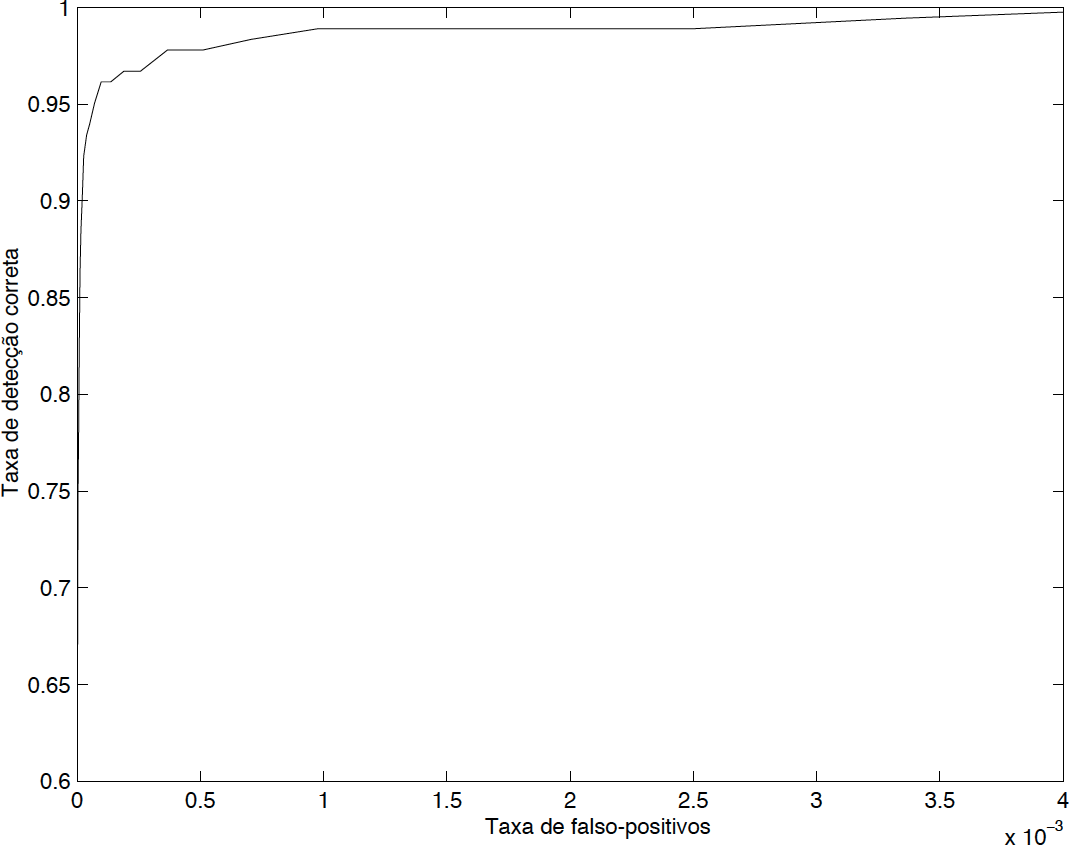
\includegraphics[height=0.6\textheight,width=0.8\textwidth]{imagens/roc_200_features.png}};
    \begin{scope}[x={(image.south east)},y={(image.north west)}]
        %\draw[help lines,xstep=.1,ystep=.1] (0,0) grid (1,1);
        %\foreach \x in {0,1,...,9} { \node [anchor=north] at (\x/10,0) {0.\x}; }
        %\foreach \y in {0,1,...,9} { \node [anchor=east] at (0,\y/10) {0.\y}; }
        \draw[red] (0.6,0.6) node {Não é bom o suficiente!};
        \draw[red] (0.6,0.4) node {Nem tempo real};
    \end{scope}
\end{tikzpicture}
\end{center}

\end{frame}


%SUBSEC%%%%%%%%%%%%%%%%%%%%%%%%%%%%%%%%%%%%%%%%%%%%%%%
\subsubsection{Classificadores em Cascata}

%FRAME%%%%%%%%%%%%%%%%%%%%%%%%%%%%%%%%%%%%%%%%%%%%%%%
\begin{frame}[fragile]{Classificadores em Cascata}
\begin{itemize}
    \item Gasta tempo apenas com faces em potencial
    \item Classificador de duas características: quase 100\% de detecção com 50\% de falso-positivos. Pode ser o primeiro estágio da cascata
    \item Uma subjanela que falha em qualquer estágio é imediatamente rejeitada
\end{itemize}

\begin{adjustbox}{max width=\textwidth}
\begin{tikzpicture}[
    font=\scriptsize,
    node distance= 4cm and 3cm,
    arrow/.style = {thick,
                    -stealth},
    decision/.style = {minimum width=#1,
                       diamond, aspect=1.5,
                       text centered,
                       align=center,
                       draw=black},
    process/.style = {minimum width=#1,
                      rectangle,
                      text centered,
                      draw=black},
    startstop/.style = {minimum width=#1,
                        rectangle,
                        rounded corners,
                        text centered,
                        draw=black},
    ]
    
    \node (subjanela) [startstop=5mm] {Subjanela};
    \node (estagio1)  [decision=5mm, right of=subjanela] {Estágio 1\\Face?};
    \node (estagio2)  [decision=5mm, right of=estagio1]  {Estágio 2\\Face?};
    \node (estagio3)  [decision=5mm, right of=estagio2]  {Estágio 3\\Face?};
    \node (detecta)   [process=5mm, right of=estagio3]   {Face detectada};
    
    \DistanciaCentros(estagio1,estagio3){distance}
    \node (rejeita)   [process=\distance, below of=estagio2, node distance=2.0cm]   {Subjanela rejeitada};
    
    \draw [arrow] (subjanela) -- (estagio1);
    \draw [arrow] (estagio1.east) -- node[anchor=south] {Talvez} (estagio2.west);
    \draw [arrow] (estagio2.east) -- node[anchor=south] {Talvez} (estagio3.west);
    \draw [arrow] (estagio3.east) -- node[anchor=south] {Talvez} (detecta.west);
    \draw [arrow] (estagio1.south) -- node[anchor=east] {Não!} (rejeita.north west);
    \draw [arrow] (estagio2.south) -- node[anchor=east] {Não!} (rejeita);
    \draw [arrow] (estagio3.south) -- node[anchor=east] {Não!} (rejeita.north east);
\end{tikzpicture}
\end{adjustbox}
\end{frame}

%FRAME%%%%%%%%%%%%%%%%%%%%%%%%%%%%%%%%%%%%%%%%%%%%%%%
\begin{frame}{Classificadores em Cascata}
\begin{itemize}
    \item Os estágios são progressivamente mais complexos e com menor taxa de falso-positivos
    \item A taxa de detecção da cascata é obtida multiplicando as taxas de cada estágio individual
    \item Uma cascata de 10 estágios, cada um com 99\% de detecção e um pouco menos de 30\% de falso-positivos resulta em uma taxa de detecção de 90\% e uma taxa de falso-positivos na ordem de $10^{-6}$
\end{itemize}
\end{frame}

%FRAME%%%%%%%%%%%%%%%%%%%%%%%%%%%%%%%%%%%%%%%%%%%%%%%
\begin{frame}{Classificadores em Cascata}
\begin{figure}[htbp]
%    \caption{Quatro estágios de um classificador em cascata}
    \label{fig:julio_cascade}
    \begin{subfigure}[t]{0.24\textwidth}
    \centering
    \caption{Estágio 1}
    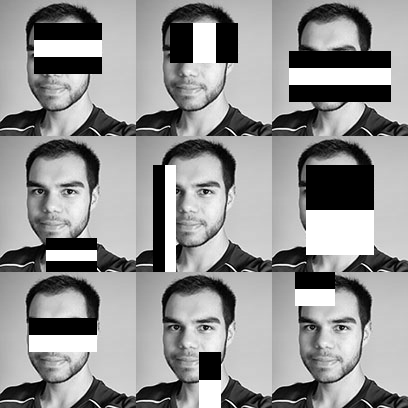
\includegraphics[height=0.6\textheight,width=\textwidth,keepaspectratio]{imagens/cascata_estagio_01.png}
    \end{subfigure}
    \begin{subfigure}[t]{0.24\textwidth}
    \centering
    \caption{Estágio 2}
    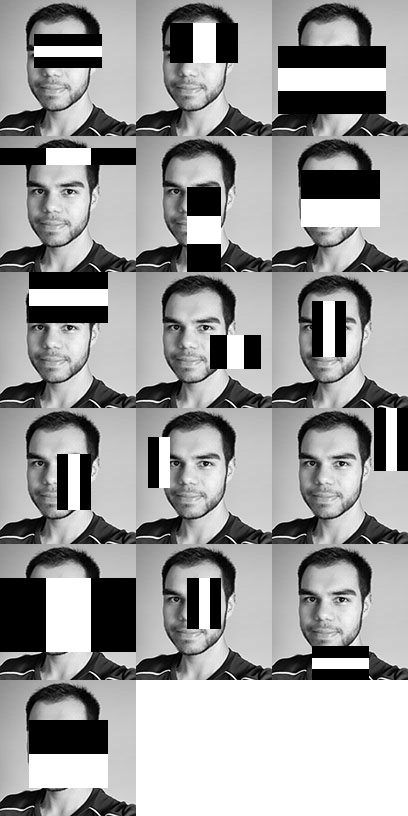
\includegraphics[height=0.6\textheight,width=\textwidth,keepaspectratio]{imagens/cascata_estagio_02.png}
    \end{subfigure}
    \begin{subfigure}[t]{0.24\textwidth}
    \centering
    \caption{Estágio 3}
    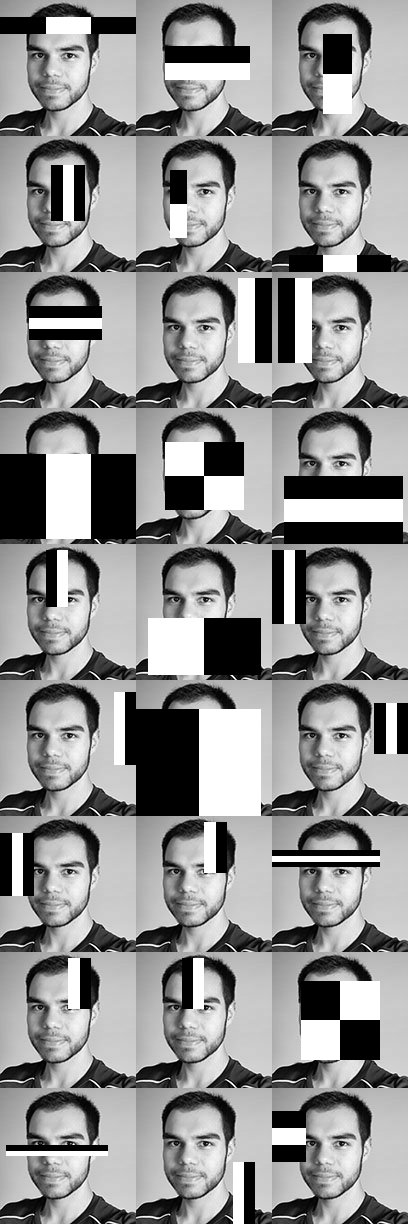
\includegraphics[height=0.6\textheight,width=\textwidth,keepaspectratio]{imagens/cascata_estagio_03.png}
    \end{subfigure}
    \begin{subfigure}[t]{0.24\textwidth}
    \centering
    \caption{Estágio 4}
    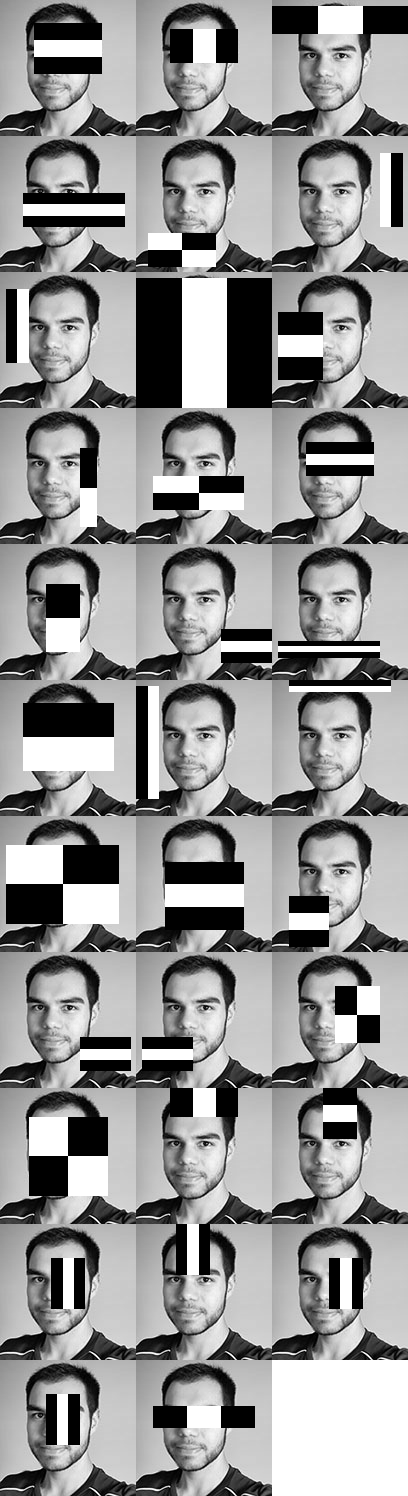
\includegraphics[height=0.6\textheight,width=\textwidth,keepaspectratio]{imagens/cascata_estagio_04.png}
    \end{subfigure}
\end{figure}
\end{frame}

%FRAME%%%%%%%%%%%%%%%%%%%%%%%%%%%%%%%%%%%%%%%%%%%%%%%
\begin{frame}{Classificadores em Cascata}
\begin{center}
\includemedia[
width=288px,
height=162px,
activate=pageopen,
addresource=imagens/VJ_detection-288x162.mp4,
flashvars={source=imagens/VJ_detection-288x162.mp4},
passcontext
]{}{VPlayer.swf}
\end{center}
\end{frame}

%FRAME%%%%%%%%%%%%%%%%%%%%%%%%%%%%%%%%%%%%%%%%%%%%%%%
\begin{frame}{FDDB Benchmark}
\begin{figure}
    \centering
    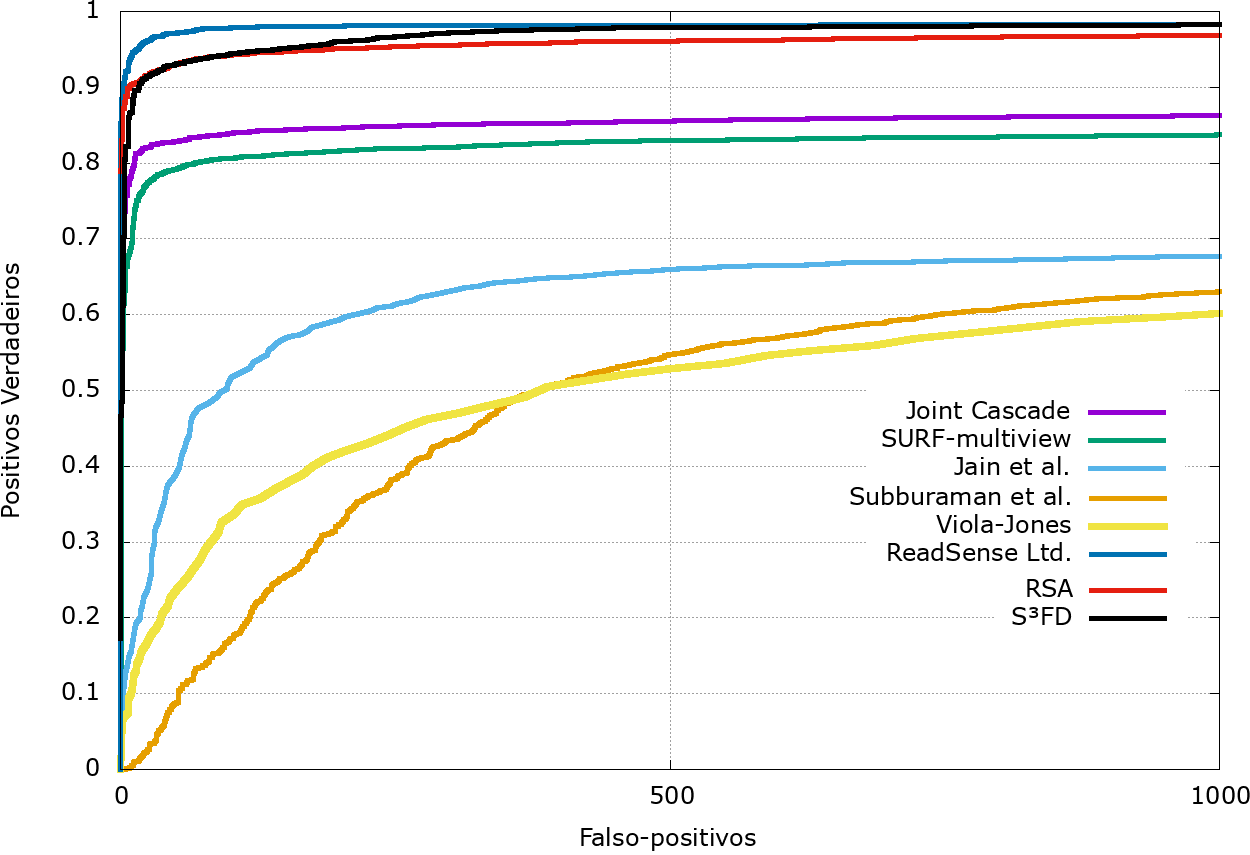
\includegraphics[height=0.82\textheight,width=\textwidth,keepaspectratio]{imagens/FDDB_deteccao_compara.png}
\end{figure}
\end{frame}


%SUBSEC%%%%%%%%%%%%%%%%%%%%%%%%%%%%%%%%%%%%%%%%%%%%%%%
\subsection{OpenCV}

%FRAME%%%%%%%%%%%%%%%%%%%%%%%%%%%%%%%%%%%%%%%%%%%%%%%
\begin{frame}{OpenCV}
Treinamento do classificador em cascata usando \texttt{opencv\_traincascade}:

\begin{itemize}
    \item 10 estágios
    \item 5000 imagens positivas
    \item 3000 imagens negativas
    \item 36$\times$36 pixels
    \item 99,5\% de detecção
    \item No máximo 50\% de falso-positivos por estágio
    \item Concluído em 1 dia 7 horas e 42 minutos
\end{itemize}

\end{frame}


%FRAME%%%%%%%%%%%%%%%%%%%%%%%%%%%%%%%%%%%%%%%%%%%%%%%
\begin{frame}[fragile]{OpenCV}
\begin{minted}[fontsize=\scriptsize]{python}
import cv2

classificador = cv2.CascadeClassifier('haarcascade_frontalface.xml')
camera = cv2.VideoCapture(0)

while camera.isOpened():
    _, imagem = camera.read()

    cinza = cv2.cvtColor(imagem, cv2.COLOR_BGR2GRAY)

    faces = classificador.detectMultiScale(
        cinza, scaleFactor=1.2, minNeighbors=5, minSize=(30, 30))

    for (x, y, w, h) in faces:
        cv2.rectangle(imagem, (x, y), (x + w, y + h), (0, 0, 255), 2)

    cv2.imshow('Detector de Faces', imagem)
\end{minted}
\end{frame}


%FRAME%%%%%%%%%%%%%%%%%%%%%%%%%%%%%%%%%%%%%%%%%%%%%%%
\begin{frame}{OpenCV}
Teste com imagens da Labeled Faces in the Wild
\begin{figure}[htbp]
%    \caption{Teste do classificador em cascata com imagens da Labeled Faces in the Wild}
    \label{fig:detector_facial_lfw}
    \begin{center}
        {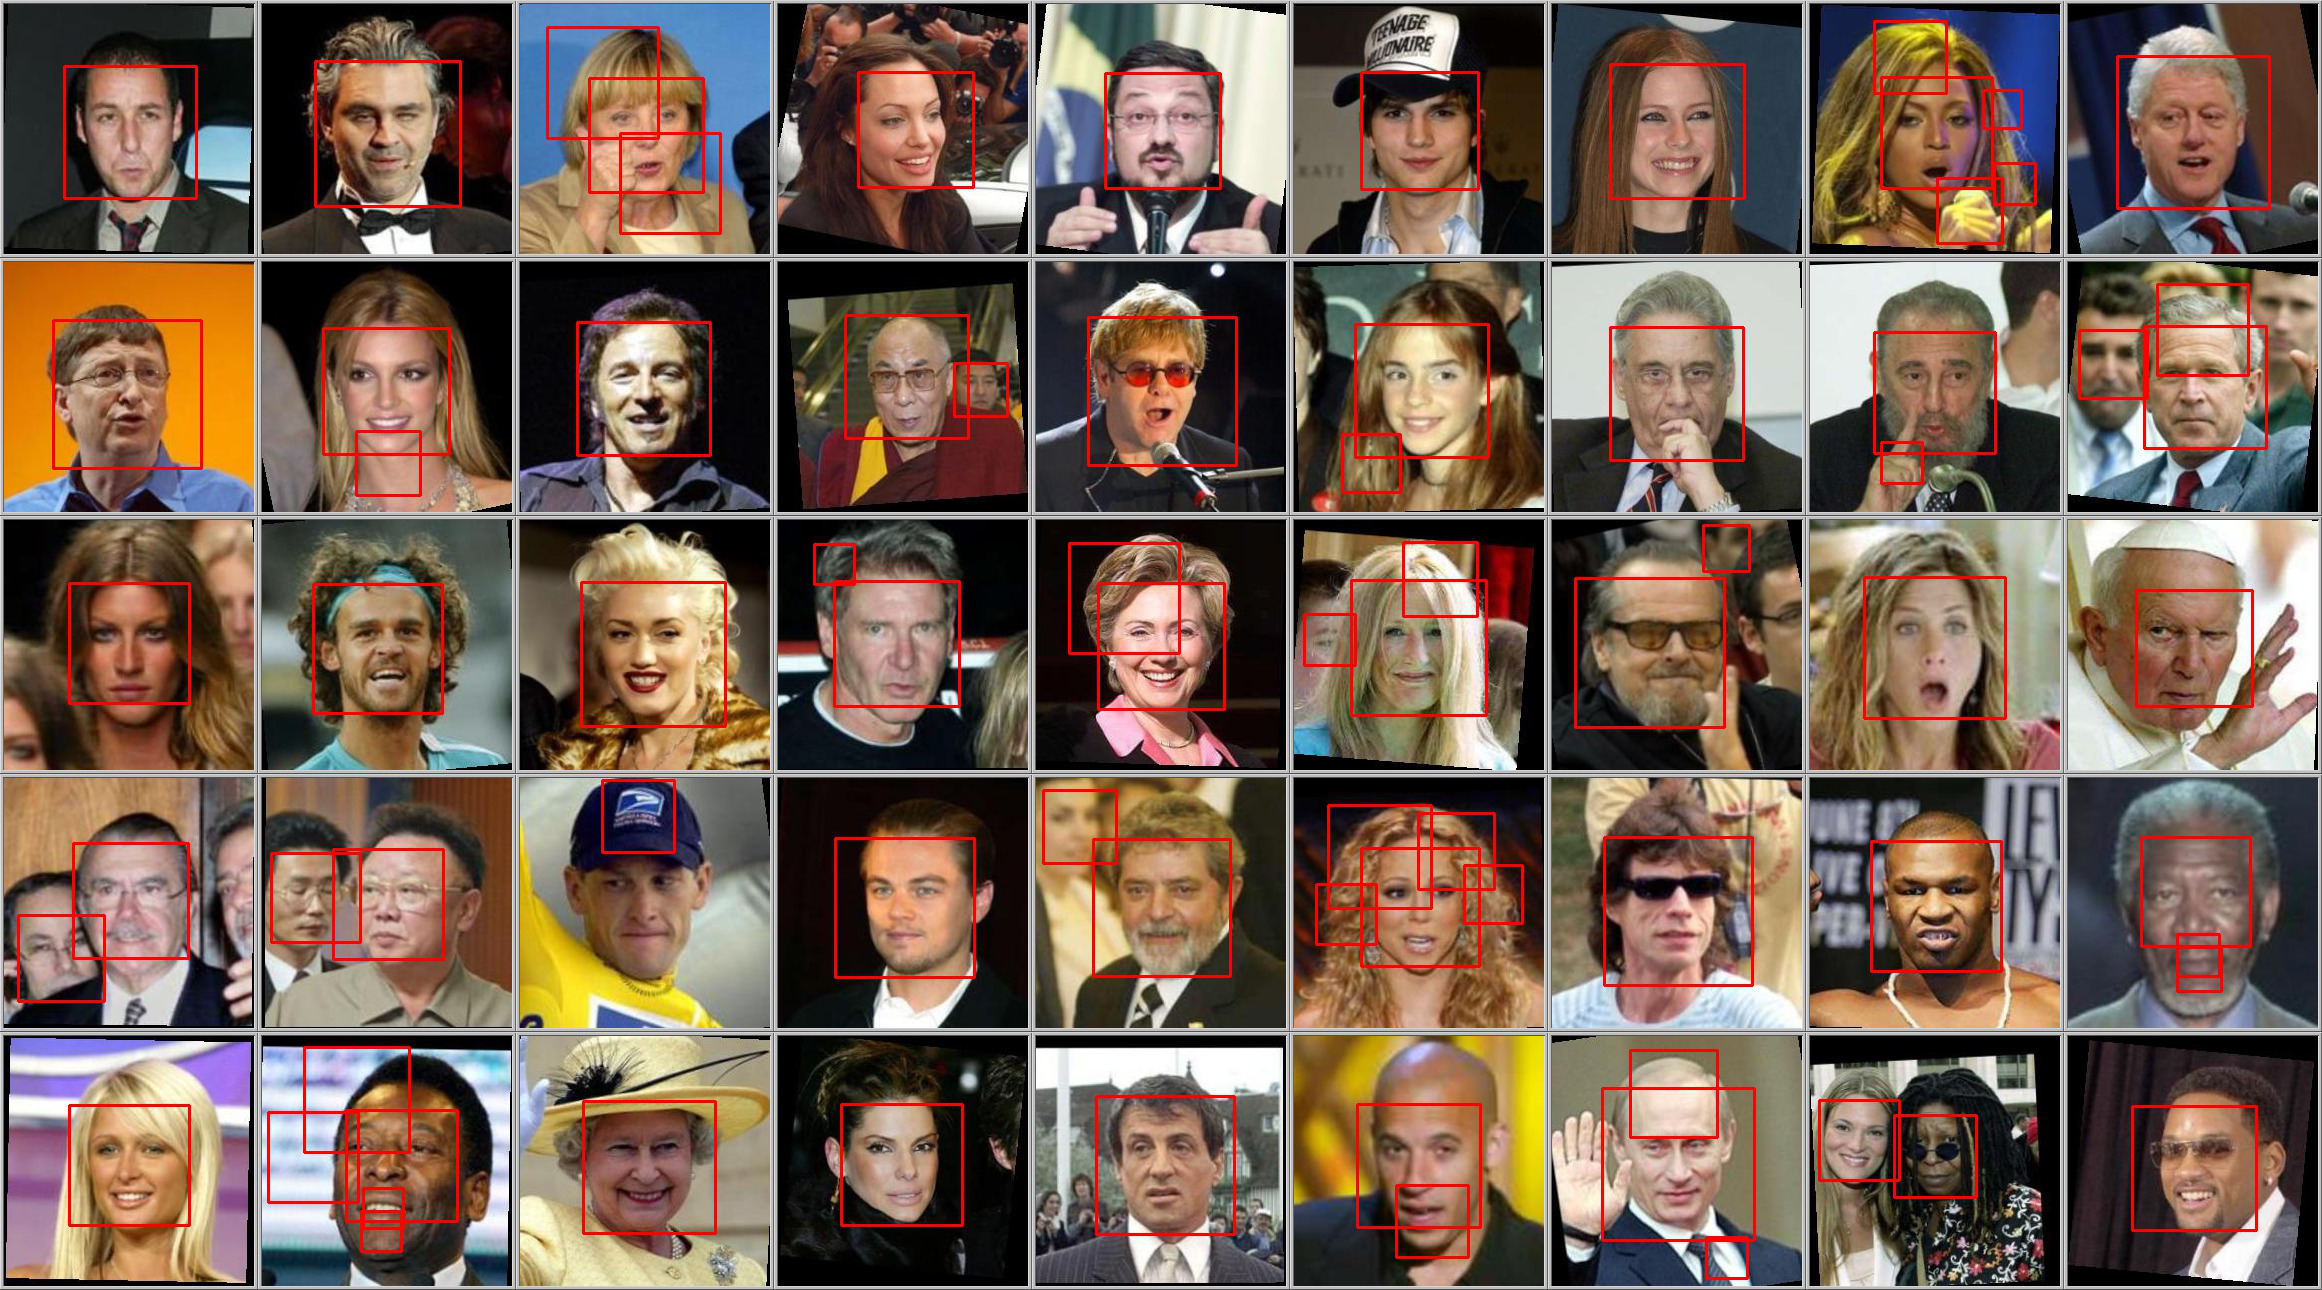
\includegraphics[width=0.99\linewidth]{imagens/detector_facial_lfw.jpg}}
    \end{center}
\end{figure}
\end{frame}
%%%%%%%%%%%%%%%%%%%%%%%%%%%%%%%%%%%%%%%%%%%%%%%%%%%%%%
%SEC%%%%%%%%%%%%%%%%%%%%%%%%%%%%%%%%%%%%%%%%%%%%%%%%%%
\section{Reconhecimento Facial}

%FRAME%%%%%%%%%%%%%%%%%%%%%%%%%%%%%%%%%%%%%%%%%%%%%%%
\begin{frame}[fragile]{Definição}
É uma tecnologia capaz de realizar:

\begin{itemize}
\item \textbf{Verificação}: dada uma face e uma alegação de identidade, informa se a face realmente pertence ao indivíduo.  

\item \textbf{Identificação}: compara a imagem de uma face desconhecida com todas as imagens em um banco de dados para determinar sua identidade.
\end{itemize}
\begin{figure}[htbp]
%    \caption{Etapas do reconhecimento facial}
    \label{fig:etapas_reconhecimento}
    \begin{adjustbox}{max width=\textwidth}
    \begin{tikzpicture}[
        font=\scriptsize, node distance=2cm,
        mynode/.style={draw, text width=2.5cm, align=center}
        ]
        \node[align=center] (input) {Imagem/\\Vídeo};
        \node[mynode,right=0.5cm of input] (detec) {Detecção\\Facial};
        \node[mynode,right=of detec] (extra) {Extração de\\Características};
        \node[mynode,right=of extra] (recon) {Reconhecimento\\Facial};
        \node[align=center,right=0.5cm of recon] (ident) {Identificação/\\Verificação};
        
        \draw[->,shorten <=1pt,shorten >=1pt] (input) -- (detec);
        \draw[->,shorten <=1pt,shorten >=1pt] (detec) -- node[fill=white] {Faces}(extra);
        \draw[->,shorten <=1pt,shorten >=1pt] (extra) -- node[fill=white] {Modelo}(recon);
        \draw[->,shorten <=1pt,shorten >=1pt] (recon) -- (ident);
    \end{tikzpicture}
    \end{adjustbox}
\end{figure}
\end{frame}


%FRAME%%%%%%%%%%%%%%%%%%%%%%%%%%%%%%%%%%%%%%%%%%%%%%%
\begin{frame}{Técnicas}
\begin{itemize}
\item Eigenfaces (PCA)
\item Fisherfaces (LDA)
\item Local Binary Patterns (LBP)
\item Filtros de Gabor
\item GaussianFace (DGP-LVM)
\item Redes Neurais Profundas (DNN)
\end{itemize}
\end{frame}

%SUBSEC%%%%%%%%%%%%%%%%%%%%%%%%%%%%%%%%%%%%%%%%%%%%%%%
\subsection{PCA}

%FRAME%%%%%%%%%%%%%%%%%%%%%%%%%%%%%%%%%%%%%%%%%%%%%%%
\begin{frame}{Espaço das imagens de faces}
\begin{itemize}
\item Uma imagem de $100\times100$ pixels pode ser representada como um vetor de 10000 dimensões
\item Apenas um pequeno grupo desses vetores correspondem a faces
\item É possível representar essas faces em um subespaço de dimensão reduzida
\item Os principais métodos de redução de dimensionalidade são o PCA e o LDA
\end{itemize}
\end{frame}


%FRAME%%%%%%%%%%%%%%%%%%%%%%%%%%%%%%%%%%%%%%%%%%%%%%%
\begin{frame}{Análise de Componentes Principais (PCA)}
\begin{itemize}
\item É uma técnica que converte um conjunto de observações de variáveis possivelmente correlacionadas em um conjunto de valores linearmente não correlacionados, chamados de componentes principais
\item O primeiro componente principal é o que possui a maior variância
\item Cada componente seguinte possui a máxima variância e é ortogonal aos compoentes anteriores
\end{itemize}
\end{frame}


%FRAME%%%%%%%%%%%%%%%%%%%%%%%%%%%%%%%%%%%%%%%%%%%%%%%
\begin{frame}{Análise de Componentes Principais (PCA)}
\begin{figure}[htbp]
%    \caption{Análise de Componentes Principais}
    \label{fig:pca}
    \begin{subfigure}[t]{0.48\textwidth}
    \caption{Distribuição original}
    \centering
    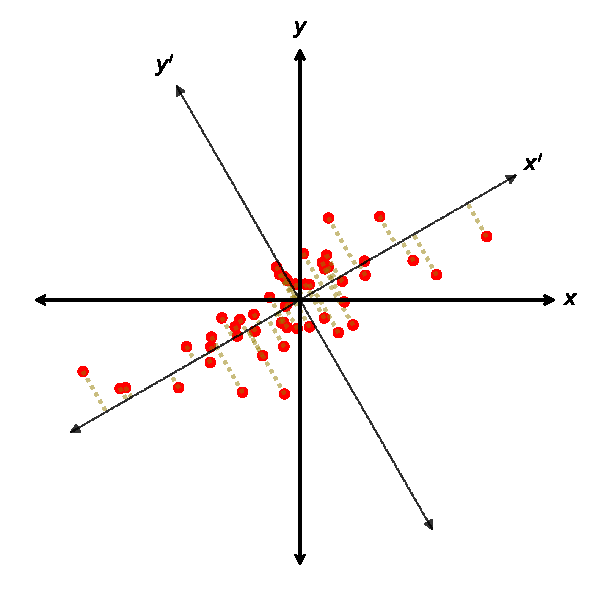
\includegraphics[width=\textwidth]{imagens/pca1.pdf}
    \end{subfigure}
    \begin{subfigure}[t]{0.48\textwidth}
    \caption{Apenas 1\textordmasculine componente principal}
    \centering
    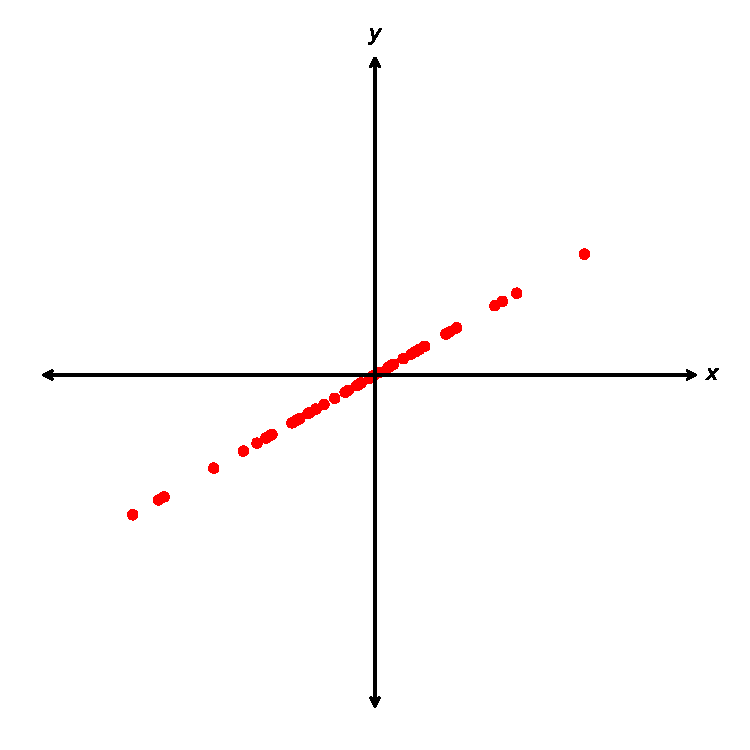
\includegraphics[width=\textwidth]{imagens/pca2.pdf}
    \end{subfigure}
\end{figure}
\end{frame}

%SUBSEC%%%%%%%%%%%%%%%%%%%%%%%%%%%%%%%%%%%%%%%%%%%%%%%
\subsection{Eigenfaces}

%FRAME%%%%%%%%%%%%%%%%%%%%%%%%%%%%%%%%%%%%%%%%%%%%%%%
\begin{frame}{Eigenfaces}
\begin{itemize}
    \item Método desenvolvido por \citeonline{turk1991eigenfaces}
    \item Eigenfaces são os componentes principais de uma distribuição de faces
    \item Cada face pode ser representada como uma combinação linear de eigenfaces
\end{itemize}
\begin{figure}[htbp]
    \centering
%    \caption{Representação de uma face como combinação linear de eigenfaces}
    \label{fig:eigenfaces_comblinear}
    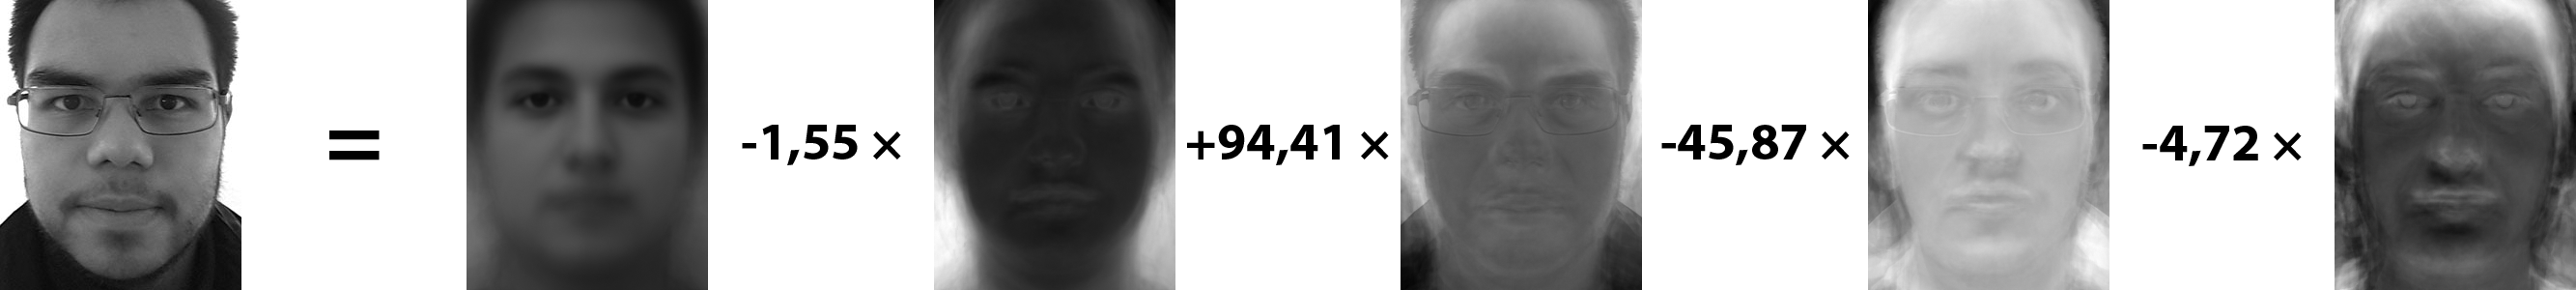
\includegraphics[width=0.95\linewidth]{imagens/eign_lincomb.png}
\end{figure}
\end{frame}


%FRAME%%%%%%%%%%%%%%%%%%%%%%%%%%%%%%%%%%%%%%%%%%%%%%%
\begin{frame}{Eigenfaces}
Algoritmo:
\begin{enumerate}
    \item Obter $M$ imagens $I_1, I_2, I_3 \ldots I_M$ com dimensão $N \times N$.
    As imagens devem estar centralizadas.
    \item Representar cada imagem $I_i$ como um vetor $\Gamma_i$ de dimensão $N^2 \times 1$.
    %
    \begin{equation*} \label{eq:eign_gamma}
        \begin{bmatrix}
        a_{11} & a_{12} & \cdots & a_{1N}\\ 
        a_{21} & a_{22} & \cdots & a_{2N}\\ 
        \vdots & \vdots & \ddots & \vdots\\ 
        a_{N1} & a_{N1} & \cdots & a_{NN}
        \end{bmatrix}_{N \times N} \rightarrow \begin{bmatrix}
        a_{11}\\ 
        \vdots\\ 
        a_{1N}\\ 
        \vdots\\ 
        a_{2N}\\
        \vdots\\ 
        a_{NN}
        \end{bmatrix}_{N^2 \times 1}
    \end{equation*}
    %
    \seti
\end{enumerate}
\end{frame}


%FRAME%%%%%%%%%%%%%%%%%%%%%%%%%%%%%%%%%%%%%%%%%%%%%%%
\begin{frame}{Eigenfaces}
\begin{enumerate}
    \conti
    \item Calcular o vetor $\Psi$ correspondente à face média.
    %
    \begin{equation*} \label{eq:eign_media}
        \Psi = \frac{1}{M}\sum_{i=1}^{M}\Gamma_i
    \end{equation*}
    %
    \item Subtrair a face média de cada vetor $\Gamma_i$ para obter o conjunto de vetores $\Phi_i$.
    %
    \begin{equation*} \label{eq:eign_phi}
        \Phi_i = \Gamma_i - \Psi
    \end{equation*}
    %
    \item Encontrar a matriz $C$ de covariância.
    %
    \begin{equation*} \label{eq:eign_c}
        C = AA^T \text{, onde } A = \begin{bmatrix}\Phi_1  & \Phi_2 & \ldots  & \Phi_3\end{bmatrix}
    \end{equation*}
    %
    $C$ é uma matriz $N^2 \times N^2$ e $A$ é uma matriz $N^2 \times M$.
    \seti
\end{enumerate}
\end{frame}


%FRAME%%%%%%%%%%%%%%%%%%%%%%%%%%%%%%%%%%%%%%%%%%%%%%%
\begin{frame}{Eigenfaces}
\begin{enumerate}
    \conti
    \item Calcular os autovetores $u_i$ de $C = AA^T$.
    
    Em vez desse cálculo, que resultaria em $N^2$ autovetores, calcular os autovetores $v_i$ da matriz $A^TA$ de dimensão $M \times M$.
    %
    \begin{equation*} \label{eq:eign_autov}
    \begin{alignedat}{2}
                     && A^T Av_i    &= \mu_i v_i\\
    \Rightarrow\quad && AA^T Av_i   &= \mu_i Av_i\\
    \Rightarrow\quad && CAv_i       &= \mu_i Av_i\\
    \Rightarrow\quad && u_i         &= Av_i
    \end{alignedat}
    \end{equation*}
    %
    ou seja, $Av_i$ são autovetores de $C = AA^T$. Os $M$ autovalores de $A^TA$ correspondem aos $M$ maiores autovalores de $AA^T$.
    \item Manter apenas os $K$ autovetores, correspondentes aos $K$ maiores autovalores.%
    \seti
\end{enumerate}
\end{frame}


%SUBSEC%%%%%%%%%%%%%%%%%%%%%%%%%%%%%%%%%%%%%%%%%%%%%%%
\subsection{OpenCV}

%FRAME%%%%%%%%%%%%%%%%%%%%%%%%%%%%%%%%%%%%%%%%%%%%%%%
\begin{frame}[fragile]{OpenCV}
\begin{minted}[fontsize=\small]{python}
# Obtém imagens de treino com ids e nomes
imgs, ids, nomes = le_imagens_de_treino(dir_treino)

# Treina o reconhecedor de faces
reconhecedor = cv2.face.EigenFaceRecognizer_create(300)
reconhecedor.train(np.asarray(imgs),np.asarray(ids))

# Realiza o reconhecimento
cinza = cv2.imread(foto, cv2.IMREAD_GRAYSCALE)
num, confianca = reconhecedor.predict(cinza)
nome = nomes[num]
\end{minted}
\end{frame}


%FRAME%%%%%%%%%%%%%%%%%%%%%%%%%%%%%%%%%%%%%%%%%%%%%%%
\begin{frame}{Eigenfaces}

\begin{figure}[htbp]
    \centering
%    \caption{Eigenfaces}
    \label{fig:eigenfaces_faces}
    \begin{subfigure}[t]{0.3\textwidth}
    \centering
    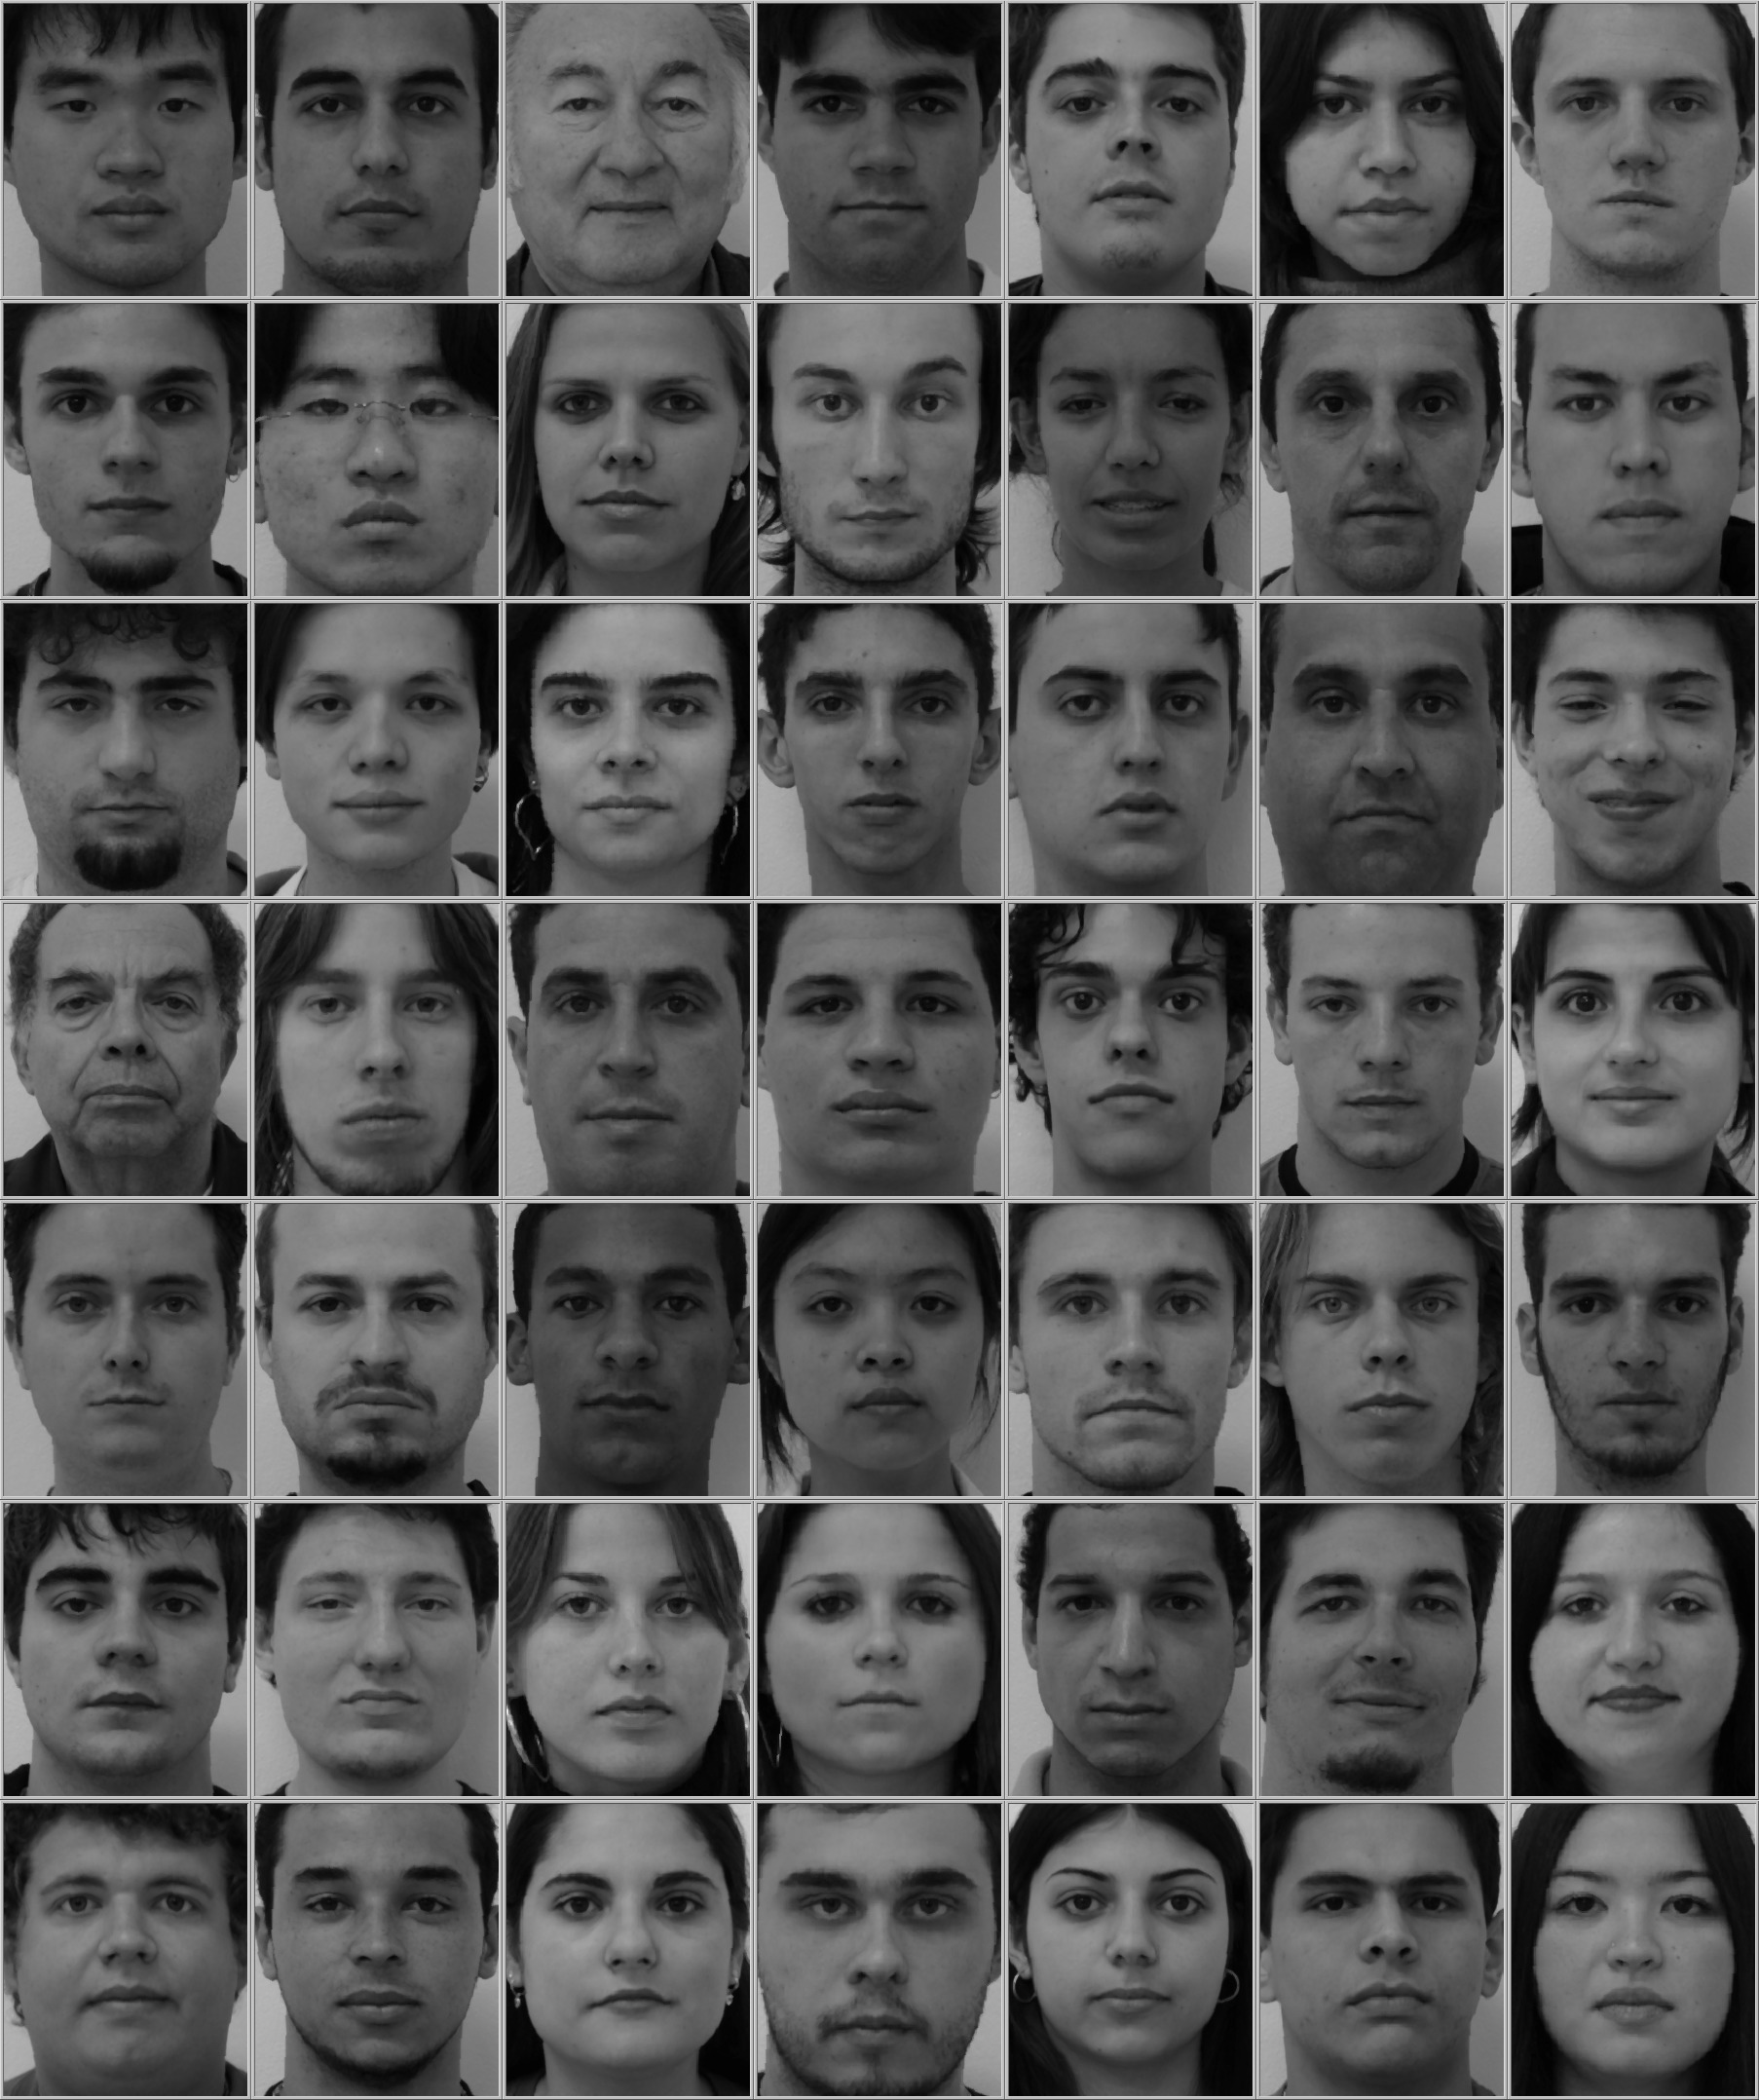
\includegraphics[width=\textwidth]{imagens/faces_fei.jpg}
    \caption{FEI Face Database}
    \end{subfigure}
    \begin{subfigure}[t]{0.3\textwidth}
    \centering
    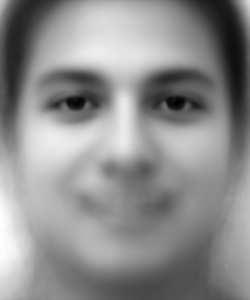
\includegraphics[width=\textwidth]{imagens/face_media.png}
    \caption{Face média}
    \end{subfigure}
    \begin{subfigure}[t]{0.3\textwidth}
    \centering
    
\includegraphics[width=\textwidth]{imagens/eigenfaces.png}
    \caption{Eigenfaces}
    \end{subfigure}
\end{figure}
\end{frame}


%FRAME%%%%%%%%%%%%%%%%%%%%%%%%%%%%%%%%%%%%%%%%%%%%%%%
\begin{frame}{Eigenfaces}
\begin{figure}[htbp]
    \centering
    \caption{Teste com o banco de faces FERET}
    \label{fig:eigenfaces_resultado_feret}
    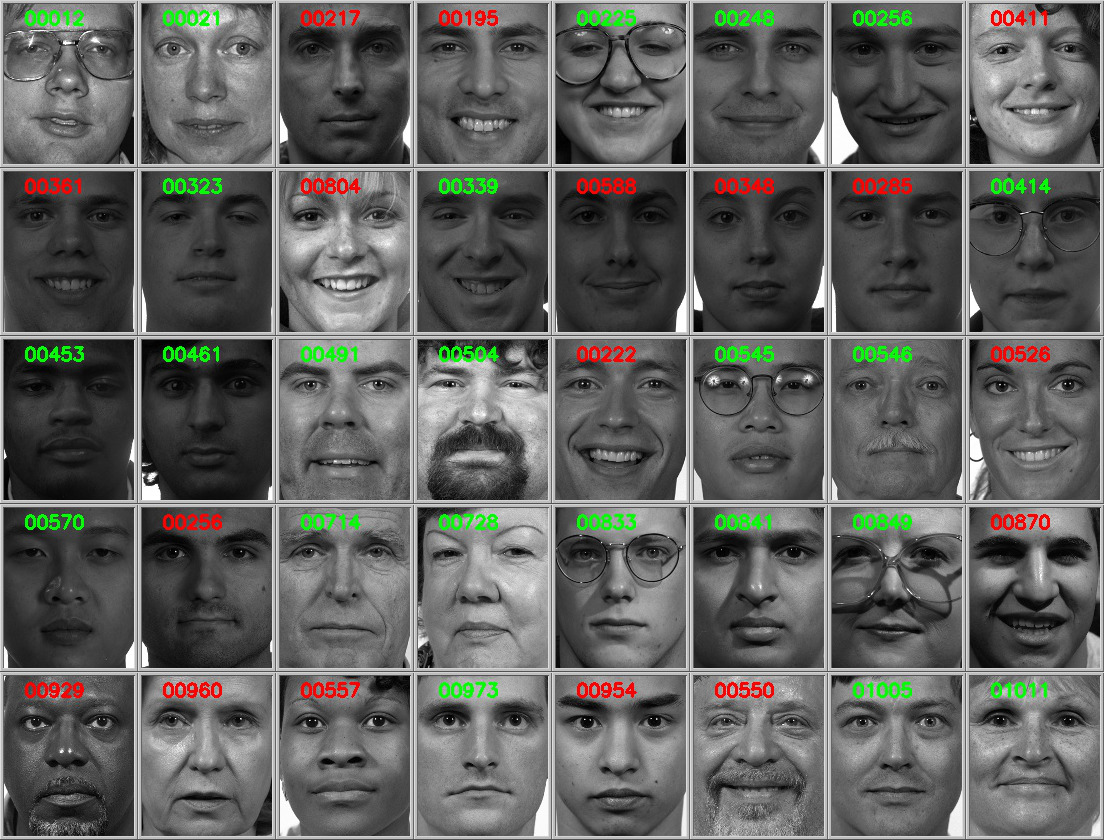
\includegraphics[width=0.8\linewidth]{imagens/eigenfaces_resultado_feret.jpg}
\end{figure}
\end{frame}


%FRAME%%%%%%%%%%%%%%%%%%%%%%%%%%%%%%%%%%%%%%%%%%%%%%%
\begin{frame}{Eigenfaces}
\begin{table}[htpb]
\centering
\caption{Bancos de faces utilizados para testes}
\label{tab:bancos_faces}
\begin{tabular}{|l|l|l|}
\hline
\textbf{Banco de faces} & \textbf{Indivíduos} & \textbf{Fotos de treino} \\\hline
\textbf{AT\&T}          & 40                  & 360                      \\\hline
\textbf{FERET}          & 865                 & 1542                     \\\hline
\textbf{Extended Yale}  & 38                  & 1862                     \\\hline
\end{tabular}
\end{table}
\end{frame}


%FRAME%%%%%%%%%%%%%%%%%%%%%%%%%%%%%%%%%%%%%%%%%%%%%%%
\begin{frame}{Eigenfaces}
\begin{table}[htbp]
\centering
\caption{Comparação dos algoritmos de reconhecimento facial}
\label{tab:compara_reconhecimento}
\begin{tabular}{|c|l|l|}
\hline
\textbf{Método}                       & \textbf{Banco de faces} & \textbf{Taxa de acertos} \\\hline
\multirow{3}{*}{\textbf{Eigenfaces}}  & AT\&T                   & 95,0\%                   \\
                                      & FERET                   & 63,4\%                   \\
                                      & Extended Yale           & 81,6\%                   \\\hline
\multirow{3}{*}{\textbf{Fisherfaces}} & AT\&T                   & 97,5\%                   \\
                                      & FERET                   & -                        \\
                                      & Extended Yale           & 100\%                    \\\hline
\multirow{3}{*}{\textbf{LBPH}}        & AT\&T                   & 100\%                    \\
                                      & FERET                   & 90,7\%                   \\
                                      & Extended Yale           & 94,7\%                   \\\hline
\end{tabular}
\end{table}
\end{frame}
%%%%%%%%%%%%%%%%%%%%%%%%%%%%%%%%%%%%%%%%%%%%%%%%%%%%%%
%SEC%%%%%%%%%%%%%%%%%%%%%%%%%%%%%%%%%%%%%%%%%%%%%%%%%%
\section{Implementação do Projeto}


%FRAME%%%%%%%%%%%%%%%%%%%%%%%%%%%%%%%%%%%%%%%%%%%%%%%
\begin{frame}{Implementação do Projeto}
O projeto é dividido em dois módulos:
\medskip
\begin{itemize}
    \item \textbf{Módulo 1}: Captura fotos, detecta faces e envia as faces para o segundo módulo
    \item \textbf{Módulo 2}: Verifica se a mesma face já foi analisada no passado e extrai características como idade, emoções e gênero
\end{itemize}
\end{frame}


%SUBSEC%%%%%%%%%%%%%%%%%%%%%%%%%%%%%%%%%%%%%%%%%%%%%%%
\subsection{Módulo 1}

%FRAME%%%%%%%%%%%%%%%%%%%%%%%%%%%%%%%%%%%%%%%%%%%%%%%
\begin{frame}{Módulo 1: Raspberry Pi}
\begin{itemize}
    \item É um computador de placa única de baixo custo
    \item Processador quad-core 64-bit de 1,4 GHz
    \item 1 GB de memória SDRAM
    \item Interface CSI para câmera
    \item Wifi e Ethernet
    \item Roda Linux ARM
\end{itemize}
\centerline{\noindent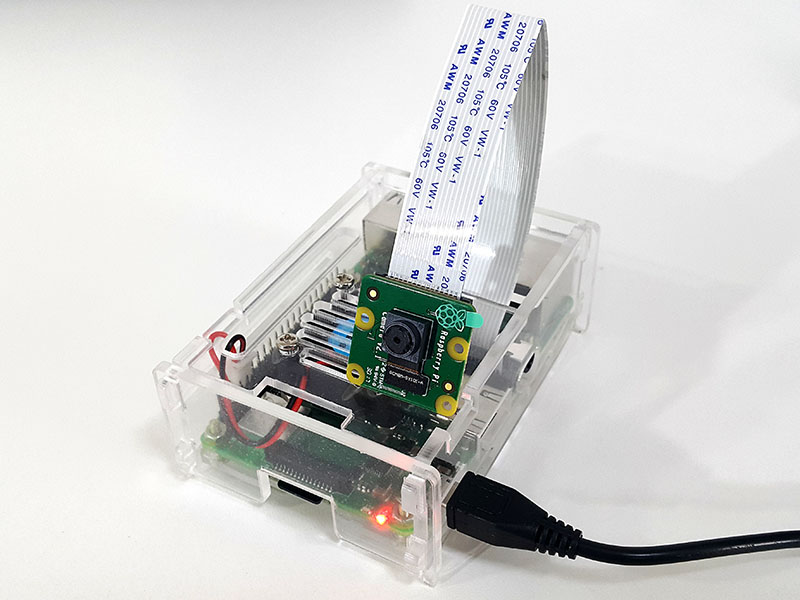
\includegraphics[width=0.45\linewidth]{raspberry.jpg}}
\end{frame}


%FRAME%%%%%%%%%%%%%%%%%%%%%%%%%%%%%%%%%%%%%%%%%%%%%%%
\begin{frame}{Módulo 1: Raspberry Pi}
\begin{itemize}
    \item Será instalado em pontos estratégicos da loja
    \item Realiza detecção utilizando o algoritmo de Viola-Jones implementado na OpenCV
    \item Envia apenas as imagens das faces para o segundo módulo para reduzir o tráfego de dados e as chamadas para a API
\end{itemize}
\end{frame}


%SUBSEC%%%%%%%%%%%%%%%%%%%%%%%%%%%%%%%%%%%%%%%%%%%%%%%
\subsection{Módulo 2}

%SUBSEC%%%%%%%%%%%%%%%%%%%%%%%%%%%%%%%%%%%%%%%%%%%%%%%
\subsubsection{Microsoft Face API}

%FRAME%%%%%%%%%%%%%%%%%%%%%%%%%%%%%%%%%%%%%%%%%%%%%%%
\begin{frame}{Módulo 2: Microsoft Face API}
\begin{itemize}
    \item Parte do Microsoft Azure Cognitive Services
    \item Realiza detecção, reconhecimento, agrupamento facial e extrai diversas outras características como emoção, idade, sexo, cor do cabelo, barba, maquiagem e uso de acessórios
    \item Grátis até 30000 transações por mês
    \item Aproximadamente R\$~3 a cada 1000 transações
\end{itemize}
\end{frame}

%FRAME%%%%%%%%%%%%%%%%%%%%%%%%%%%%%%%%%%%%%%%%%%%%%%%
\begin{frame}{Módulo 2: Microsoft Face API}
\begin{figure}[htbp]
%    \caption{Teste da Microsoft Face API}
    \label{fig:face_api_test1}
    \centering
    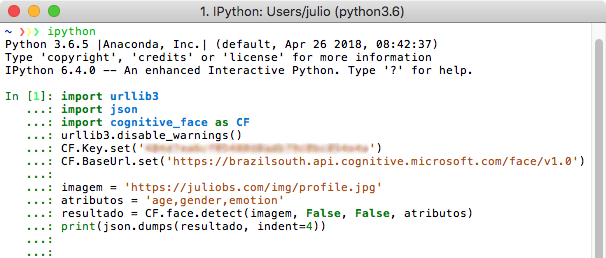
\includegraphics[height=0.8\textheight,width=\textwidth,keepaspectratio]{imagens/msft_face_api_json_1.png}
\end{figure}
\end{frame}


%FRAME%%%%%%%%%%%%%%%%%%%%%%%%%%%%%%%%%%%%%%%%%%%%%%%
\begin{frame}{Microsoft Face API}
\begin{figure}[htbp]
%    \caption{Teste da Microsoft Face API}
    \label{fig:face_api_test2}
    \begin{subfigure}[c]{0.48\textwidth}
    \centering
    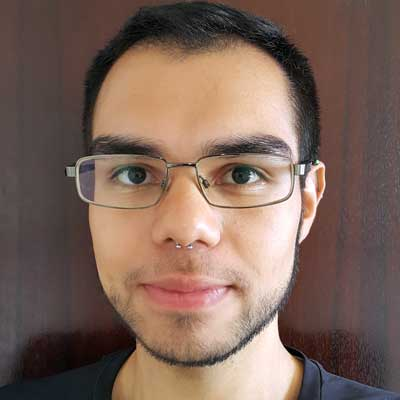
\includegraphics[height=\textheight,width=\textwidth,keepaspectratio]{imagens/profile.jpg}
    \end{subfigure}
    \begin{subfigure}[c]{0.48\textwidth}
    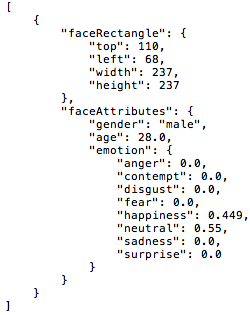
\includegraphics[height=\textheight,width=\textwidth,keepaspectratio]{imagens/msft_face_api_json_2.png}
    \end{subfigure}
\end{figure}
\end{frame}


%FRAME%%%%%%%%%%%%%%%%%%%%%%%%%%%%%%%%%%%%%%%%%%%%%%%
\begin{frame}{Microsoft Face API}
\begin{figure}[htbp]
    \caption{Python SDK para a Microsoft Face API}
    \centering
    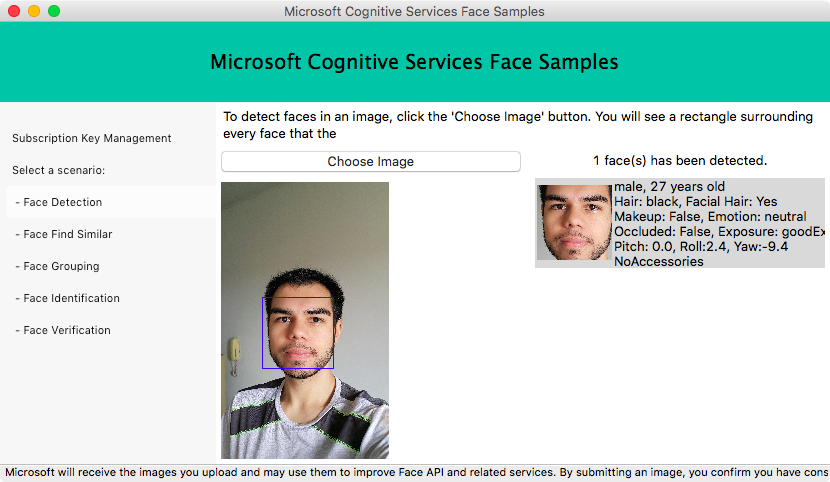
\includegraphics[width=0.8\linewidth]{imagens/msft_face_api_test.png}
\end{figure}
\end{frame}
%%%%%%%%%%%%%%%%%%%%%%%%%%%%%%%%%%%%%%%%%%%%%%%%%%%%%%
%SEC%%%%%%%%%%%%%%%%%%%%%%%%%%%%%%%%%%%%%%%%%%%%%%%%%%
\section{Conclusões}

%FRAME%%%%%%%%%%%%%%%%%%%%%%%%%%%%%%%%%%%%%%%%%%%%%%%
\begin{frame}{Conclusões}
\begin{itemize}
    \item O algoritmo de Viola-Jones é eficiente para detectar faces
    \item A biblioteca OpenCV possui diversos algoritmos implementados e facilita o desenvolvimento de aplicações
    \item A taxa de acertos do Eigenfaces é baixa quando comparada a outros métodos
    \item Reconhecimento facial irrestrito ainda é um desafio por fatores como iluminação, baixa resolução, variação de pose, oclusão e expressão facial
    \item Soluções comerciais, como a Face API da Microsoft, oferecem o estado da arte em diversas tarefas como detecção facial, reconhecimento facial, detecção de emoções e identificação de gênero
    \item É possível utilizar o Raspberry Pi como uma solução barata de câmera inteligente
\end{itemize}
\end{frame}


%FRAME%%%%%%%%%%%%%%%%%%%%%%%%%%%%%%%%%%%%%%%%%%%%%%%
\begin{frame}{Trabalhos Futuros}
\begin{itemize}
    \item Treinar um classificador com menos falso-positivos
    \item Estudar novos métodos de reconhecimento facial e extração de características para substituir a Face API da Microsoft
\end{itemize}
\end{frame}


%FRAME%%%%%%%%%%%%%%%%%%%%%%%%%%%%%%%%%%%%%%%%%%%%%%%
\begin{frame}{Trabalhos Futuros}
\begin{itemize}
    \item Criar um dashboard com gráficos e tabelas que facilitem a tomada de decisões utilizando as informações coletadas
\end{itemize}
\begin{figure}[htbp]
%    \caption{Teste da Microsoft Face API}
    \label{fig:tableau}
    \centering
    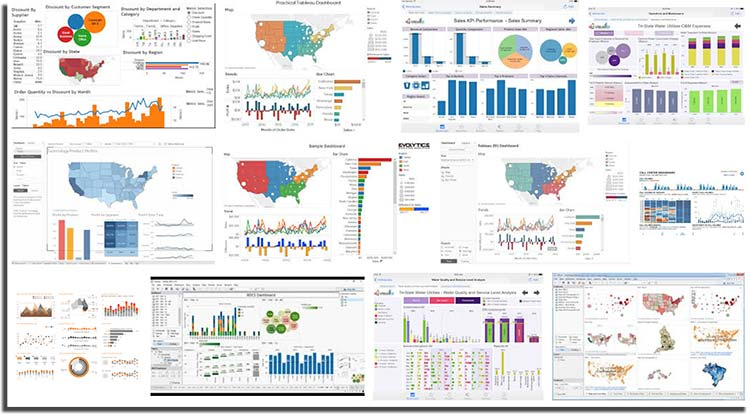
\includegraphics[height=0.7\textheight,width=\textwidth,keepaspectratio]{imagens/tableau.jpg}
\end{figure}
\end{frame}

%%%%%%%%%%%%%%%%%%%%%%%%%%%%%%%%%%%%%%%%%%%%%%%%%%%%%%
%SEC%%%%%%%%%%%%%%%%%%%%%%%%%%%%%%%%%%%%%%%%%%%%%%%%%%
\section{Referências}

%FRAME%%%%%%%%%%%%%%%%%%%%%%%%%%%%%%%%%%%%%%%%%%%%%%%
\begin{frame}[allowframebreaks]{Referências}
    \bibliography{referencias}
\end{frame}

\end{document}